%%%%%%%%%%%%%%%%%%%%%%%%%%%%%%%%%%%%%%%%%
% Masters/Doctoral Thesis 
% LaTeX Template
% Version 1.43 (17/5/14)
%
% This template has been downloaded from:
% http://www.LaTeXTemplates.com
%
% Original authors:
% Steven Gunn 
% http://users.ecs.soton.ac.uk/srg/softwaretools/document/templates/
% and
% Sunil Patel
% http://www.sunilpatel.co.uk/thesis-template/
%
% License:
% CC BY-NC-SA 3.0 (http://creativecommons.org/licenses/by-nc-sa/3.0/)
%
% Note:
% Make sure to edit document variables in the Thesis.cls file
%
%%%%%%%%%%%%%%%%%%%%%%%%%%%%%%%%%%%%%%%%%

%----------------------------------------------------------------------------------------
%	PACKAGES AND OTHER DOCUMENT CONFIGURATIONS
%----------------------------------------------------------------------------------------

\documentclass[11pt, oneside]{Thesis} % The default font size and one-sided printing (no margin offsets)

\graphicspath{{Pictures/},{Figures/}} % Specifies the directory where pictures are stored

%\usepackage[square, authoryear, comma, sort&compress]{natbib} % Use the natbib reference package - read up on this to edit the reference style; if you want text (e.g. Smith et al., 2012) for the in-text references (instead of numbers), remove 'numbers' 
%\def\citeAuthNumYr#1{[\citeauthor{#1}, \citep{#1}, \citeyear{#1}]}

\usepackage[style=alphabetic,sorting=nyt,maxalphanames=1,doi=false]{biblatex}
\addbibresource{Bibliography.bib}

\renewcommand*{\labelalphaothers}{}

\DeclareLabelalphaTemplate{
  \labelelement{
    \field[final]{shorthand}
    \field{labelname}
    \field{label}
  }
  \labelelement{
    \literal{,\addhighpenspace}
  }
  \labelelement{
    \field{year}
  }
}

\setlength{\bibitemsep}{\baselineskip}

% Zeilenabstand auf 1.5 setzen
%\linespread{1.0}

\hypersetup{urlcolor=blue, colorlinks=true} % Colors hyperlinks in blue - change to black if annoying
\title{\ttitle} % Defines the thesis title - don't touch this

\usepackage[T1]{fontenc}
\usepackage{longtable}
\usepackage{array}
\usepackage{xcolor}
\usepackage{textcomp}
\usepackage{tikz}
\usepackage{tikz-uml}
\usepackage{graphicx}
\usepackage{float}
\usepackage{enumitem}  
\usepackage{amsmath}
\newcolumntype{P}[1]{>{\raggedright\arraybackslash}p{#1}}

\tikzumlset{fill package=gray!5}

% Listings configuration for Swift
\lstdefinelanguage{swift}
{
  morekeywords={
    func,if,then,else,for,in,while,do,switch,case,default,where,break,continue,fallthrough,return,
    typealias,struct,class,enum,protocol,var,func,let,get,set,willSet,didSet,inout,init,deinit,extension,
    subscript,prefix,operator,infix,postfix,precedence,associativity,left,right,none,convenience,dynamic,
    final,lazy,mutating,nonmutating,optional,override,required,static,unowned,safe,weak,internal,
    private,public,is,as,self,unsafe,dynamicType,true,false,nil,Type,Protocol,
  },
  morecomment=[l]{//}, % l is for line comment
  morecomment=[s]{/*}{*/}, % s is for start and end delimiter
  morestring=[b]" % defines that strings are enclosed in double quotes
}
 
\definecolor{keyword}{HTML}{BA2CA3}
\definecolor{string}{HTML}{D12F1B}
\definecolor{comment}{HTML}{008400}

\definecolor{keywordScala}{HTML}{000080}
 
\lstset{
  language=swift,
  basicstyle=\small\ttfamily,
  showstringspaces=false, % lets spaces in strings appear as real spaces
  columns=fixed,
  keepspaces=true,
  keywordstyle=\color{keyword},
  stringstyle=\color{string},
  commentstyle=\color{comment},
  breaklines=true,
  belowskip=0pt
}

% Listings configuration for Scala
% "define" Scala
\lstdefinelanguage{scala}{
  morekeywords={abstract,case,catch,class,def,%
    do,else,extends,false,final,finally,%
    for,if,implicit,import,match,mixin,%
    new,null,object,override,package,%
    private,protected,requires,return,sealed,%
    super,this,throw,trait,true,try,%
    type,val,var,while,with,yield},
  otherkeywords={=>,<-,<\%,<:,>:,\#,@param,@return},
  sensitive=true,
  morecomment=[l]{//},
  morecomment=[n]{/*}{*/},
  morestring=[b]",
  morestring=[b]',
  morestring=[b]"""
}

\lstdefinestyle{ScalaStyle}{
 keywordstyle=\color{keywordScala}
}




\begin{document}

\frontmatter % Use roman page numbering style (i, ii, iii, iv...) for the pre-content pages

\setstretch{1.3} % Line spacing of 1.3

% Define the page headers using the FancyHdr package and set up for one-sided printing
\fancyhead{} % Clears all page headers and footers
\rhead{\thepage} % Sets the right side header to show the page number
\lhead{} % Clears the left side page header

\pagestyle{fancy} % Finally, use the "fancy" page style to implement the FancyHdr headers

\newcommand{\HRule}{\rule{\linewidth}{0.5mm}} % New command to make the lines in the title page

% PDF meta-data
\hypersetup{pdftitle={\ttitle}}
\hypersetup{pdfsubject=\subjectname}
\hypersetup{pdfauthor=\authornames}
\hypersetup{pdfkeywords=\keywordnames}

% HTWG
\newcommand{\thema}{A Framework for Context-Aware Visitor Guide Systems}
\newcommand{\schlagworte}{Context-Aware Computing, Mobile Computing, Indoor Navigation, Scala, Swift, Play, Couchbase}
\newcommand{\zusammenfassung}{Lorem ipsum dolor sit amet, consetetur sadipscing elitr, sed diam nonumy eirmod tempor invidunt ut labore et dolore magna aliquyam erat, sed diam voluptua. At vero eos et accusam et justo duo dolores et ea rebum. Stet clita kasd gubergren, no sea takimata sanctus est Lorem ipsum dolor sit amet. Lorem ipsum dolor sit amet, consetetur sadipscing elitr, sed diam nonumy eirmod tempor invidunt ut labore et dolore magna aliquyam erat, sed diam voluptua. At vero eos et accusam et justo duo dolores et ea rebum. Stet clita kasd gubergren, no sea takimata sanctus est Lorem ipsum dolor sit amet. Lorem ipsum dolor sit amet, consetetur sadipscing elitr, sed diam nonumy eirmod tempor invidunt ut labore et dolore magna aliquyam erat, sed diam voluptua. At vero eos et accusam et justo duo dolores et ea rebum. Stet clita kasd gubergren, no sea takimata sanctus est Lorem ipsum dolor sit amet.}
\newcommand{\ausgabedatum}{16.10.2014}
\newcommand{\abgabedatum}{16.04.2015}
\newcommand{\autor}{Maurizio Tidei}
\newcommand{\autorStrasse}{Kapellenstr. 4}
\newcommand{\autorPLZ}{78262 }
\newcommand{\autorOrt}{Gailingen}
\newcommand{\autorGeburtsort}{Singen}
\newcommand{\autorGeburtsdatum}{23.11.1980}
\newcommand{\prueferA}{Prof. Dr. Marko Boger}
\newcommand{\prueferB}{Prof. Dr. Christian Johner}
\newcommand{\firma}{HTWG / contexagon GmbH}
\newcommand{\studiengang}{Master of Science Informatik}



\begin{titlepage}

\vspace*{-3.5cm}

\begin{flushleft}
\hspace*{-1cm} 
\includegraphics[width=15.7cm]{htwg/htwg-logo}
\end{flushleft}

\vspace{2.5cm}

\begin{center}
	\huge{
		\textbf{\thema} \\[5cm]
	}
	\Large{
		\textbf{\autor}} \\[6.5cm]
	\large{
		\textbf{Constance, \abgabedatum} \\[2.3cm]
	}
	
	\Huge{
		\textbf{{\sf MASTER'S THESIS}}
	}
\end{center}

\end{titlepage}

\thispagestyle{empty}
{
\setlength{\parskip}{0.5cm}
        \begin{center}
        \textbf{\huge MASTERARBEIT}

        \textbf{zur Erlangung des akademischen Grades}

        \textbf{\Large Master of Science (M. Sc.)}

        \textbf{an der}

        \textsf{\huge Hochschule Konstanz}\\
        {\small Technik, Wirtschaft und Gestaltung}

        \textsf{\Large Fakultät Informatik} \\
        Studiengang \studiengang
        \end{center}
}
\begin{center}

\vspace*{2cm}

\begin{tabular}{p{3cm}p{10cm}}
Thema: & \textbf{\large \thema} \\[15ex]
Masterkandidat: & \autor, \autorStrasse, \autorPLZ  \autorOrt \\[15ex]
1. Prüfer: & \prueferA \\
2. Prüfer: & \prueferB \\[25ex]
Ausgabedatum: & \ausgabedatum \\
Abgabedatum: & \abgabedatum \\
\end{tabular}
\end{center}

\begin{center}
{\Large \textbf{Zusammenfassung (Abstract)}}
\end{center}

\bigskip

\begin{center}
	\begin{tabular}{p{2.8cm}p{10cm}}
		Thema: & \thema \\
		 & \\
		Masterkandidat: & \autor \\
		 & \\
		Firma: & \firma \\
		 & \\
		Betreuer: & \prueferA  \\[.5ex]
		 &  \prueferB \\
		 & \\
		Abgabedatum: & \abgabedatum \\
		 & \\
		Schlagworte: & \schlagworte \\
		 & \\
	\end{tabular}
\end{center}

\bigskip

\noindent
\zusammenfassung
\chapter*{Ehrenwörtliche Erklärung}
\addcontentsline{toc}{chapter}{Ehrenwörtliche Erklärung}

Hiermit erkläre ich
\textit{\autor, geboren am \autorGeburtsdatum in \autorGeburtsort}, dass ich\\

\begin{tabular}{lp{12cm}}
(1) & meine Masterarbeit mit dem Titel \\[1em]
& \textbf{\thema} \\[1em]
& bei der \firma\ unter Anleitung von \prueferA\ selbständig und ohne fremde Hilfe angefertigt und keine anderen als die angeführten Hilfen benutzt habe;\\[1em]
(2) & die Übernahme wörtlicher Zitate, von Tabellen, Zeichnungen, Bildern und
Programmen aus der Literatur oder anderen Quellen (Internet) sowie die Verwendung
der Gedanken anderer Autoren an den entsprechenden Stellen innerhalb der Arbeit
gekennzeichnet habe.\\
\end{tabular}

\vspace*{1cm}

\noindent
Ich bin mir bewusst, dass eine falsche Erklärung rechtliche Folgen haben wird.\\

\vspace*{3cm}

\noindent
Konstanz, \abgabedatum \hfill \begin{tabular}{c} \\ \\ \rule{5cm}{1pt} \\ (Unterschrift)\end{tabular}


% some custom stuff
\newcommand{\smalltt}[1]{{\small\texttt{#1}}}

%----------------------------------------------------------------------------------------
%	TITLE PAGE
%----------------------------------------------------------------------------------------

%\begin{titlepage}
%\begin{center}
%
%\textsc{\LARGE \univname}\\[1.5cm] % University name
%\textsc{\Large Doctoral Thesis}\\[0.5cm] % Thesis type
%
%\HRule \\[0.4cm] % Horizontal line
%{\huge \bfseries \ttitle}\\[0.4cm] % Thesis title
%\HRule \\[1.5cm] % Horizontal line
% 
%\begin{minipage}{0.4\textwidth}
%\begin{flushleft} \large
%\emph{Author:}\\
%\href{http://www.johnsmith.com}{\authornames} % Author name - remove the \href bracket to remove the link
%\end{flushleft}
%\end{minipage}
%\begin{minipage}{0.4\textwidth}
%\begin{flushright} \large
%\emph{Supervisor:} \\
%\href{http://www.jamessmith.com}{\supname} % Supervisor name - remove the \href bracket to remove the link  
%\end{flushright}
%\end{minipage}\\[3cm]
% 
%\large \textit{A thesis submitted in fulfilment of the requirements\\ for the degree of \degreename}\\[0.3cm] % University requirement text
%\textit{in the}\\[0.4cm]
%\groupname\\\deptname\\[2cm] % Research group name and department name
% 
%{\large \today}\\[4cm] % Date
%%\includegraphics{Logo} % University/department logo - uncomment to place it
% 
%\vfill
%\end{center}
%
%\end{titlepage}

%----------------------------------------------------------------------------------------
%	DECLARATION PAGE
%	Your institution may give you a different text to place here
%----------------------------------------------------------------------------------------

%\Declaration{
%
%\addtocontents{toc}{\vspace{1em}} % Add a gap in the Contents, for aesthetics
%
%I, \authornames, declare that this thesis titled, '\ttitle' and the work presented in it are my own. I confirm that:
%
%\begin{itemize} 
%\item[\tiny{$\blacksquare$}] This work was done wholly or mainly while in candidature for a research degree at this University.
%\item[\tiny{$\blacksquare$}] Where any part of this thesis has previously been submitted for a degree or any other qualification at this University or any other institution, this has been clearly stated.
%\item[\tiny{$\blacksquare$}] Where I have consulted the published work of others, this is always clearly attributed.
%\item[\tiny{$\blacksquare$}] Where I have quoted from the work of others, the source is always given. With the exception of such quotations, this thesis is entirely my own work.
%\item[\tiny{$\blacksquare$}] I have acknowledged all main sources of help.
%\item[\tiny{$\blacksquare$}] Where the thesis is based on work done by myself jointly with others, I have made clear exactly what was done by others and what I have contributed myself.\\
%\end{itemize}
% 
%Signed:\\
%\rule[1em]{25em}{0.5pt} % This prints a line for the signature
% 
%Date:\\
%\rule[1em]{25em}{0.5pt} % This prints a line to write the date
%}
%
%\clearpage % Start a new page

%----------------------------------------------------------------------------------------
%	QUOTATION PAGE
%----------------------------------------------------------------------------------------

\pagestyle{empty} % No headers or footers for the following pages

\null\vfill % Add some space to move the quote down the page a bit

%\textit{``Thanks to my solid academic training, today I can write hundreds of words on virtually any topic without possessing a shred of information, which is how I got a good job in journalism."}

%\begin{flushright}
%Dave Barry
%\end{flushright}

\textit{\Large ``Moving on is hard, but inevitable if you don't want to be the next COBOL programmer."}

\begin{flushright}
\small From the preface to "Play for Scala" written by P.Hilton, E.Bakker, F.Canedo \cite{play-book}
\end{flushright}

\vfill\vfill\vfill\vfill\vfill\vfill\null % Add some space at the bottom to position the quote just right

\clearpage % Start a new page

%----------------------------------------------------------------------------------------
%	ABSTRACT PAGE
%----------------------------------------------------------------------------------------

%\addtotoc{Abstract} % Add the "Abstract" page entry to the Contents
%
%\abstract{\addtocontents{toc}{\vspace{1em}} % Add a gap in the Contents, for aesthetics
%
%The Thesis Abstract is written here (and usually kept to just this page). The page is kept centered vertically so can expand into the blank space above the title too\ldots
%}
%
%\clearpage % Start a new page

%----------------------------------------------------------------------------------------
%	ACKNOWLEDGEMENTS
%----------------------------------------------------------------------------------------

\setstretch{1.3} % Reset the line-spacing to 1.3 for body text (if it has changed)

\acknowledgements{\addtocontents{toc}{\vspace{1em}} % Add a gap in the Contents, for aesthetics

Lorem ipsum dolor
}
\clearpage % Start a new page

%----------------------------------------------------------------------------------------
%	LIST OF CONTENTS/FIGURES/TABLES PAGES
%----------------------------------------------------------------------------------------

\pagestyle{fancy} % The page style headers have been "empty" all this time, now use the "fancy" headers as defined before to bring them back

\lhead{\emph{Contents}} % Set the left side page header to "Contents"
\tableofcontents % Write out the Table of Contents

\lhead{\emph{List of Figures}} % Set the left side page header to "List of Figures"
\listoffigures % Write out the List of Figures

%\lhead{\emph{List of Tables}} % Set the left side page header to "List of Tables"
%\listoftables % Write out the List of Tables

%----------------------------------------------------------------------------------------
%	ABBREVIATIONS
%----------------------------------------------------------------------------------------

\clearpage % Start a new page

\setstretch{1.5} % Set the line spacing to 1.5, this makes the following tables easier to read

\lhead{\emph{Abbreviations}} % Set the left side page header to "Abbreviations"
\listofsymbols{ll} % Include a list of Abbreviations (a table of two columns)
{
\textbf{INS} & \textbf{I}nertial \textbf{N}avigation \textbf{S}ystem \\
\textbf{MEMS} & \textbf{M}icro\textbf{e}lectro\textbf{m}echanical \textbf{S}ystem \\
\textbf{DSL} & \textbf{D}omain\textbf{S}pecific\textbf{L}anguage \\
\textbf{REPL} & \textbf{R}ead-\textbf{E}val-\textbf{P}rint-\textbf{L}oop
%\textbf{Acronym} & \textbf{W}hat (it) \textbf{S}tands \textbf{F}or \\
}

%----------------------------------------------------------------------------------------
%	PHYSICAL CONSTANTS/OTHER DEFINITIONS
%----------------------------------------------------------------------------------------

%\clearpage % Start a new page
%
%\lhead{\emph{Physical Constants}} % Set the left side page header to "Physical Constants"
%
%\listofconstants{lrcl} % Include a list of Physical Constants (a four column table)
%{
%Speed of Light & $c$ & $=$ & $2.997\ 924\ 58\times10^{8}\ \mbox{ms}^{-\mbox{s}}$ (exact)\\
%% Constant Name & Symbol & = & Constant Value (with units) \\
%}

%----------------------------------------------------------------------------------------
%	SYMBOLS
%----------------------------------------------------------------------------------------

%\clearpage % Start a new page
%
%\lhead{\emph{Symbols}} % Set the left side page header to "Symbols"
%
%\listofnomenclature{lll} % Include a list of Symbols (a three column table)
%{
%$a$ & distance & m \\
%$P$ & power & W (Js$^{-1}$) \\
%% Symbol & Name & Unit \\
%
%& & \\ % Gap to separate the Roman symbols from the Greek
%
%$\omega$ & angular frequency & rads$^{-1}$ \\
%% Symbol & Name & Unit \\
%}

%----------------------------------------------------------------------------------------
%	DEDICATION
%----------------------------------------------------------------------------------------

%\setstretch{1.3} % Return the line spacing back to 1.3
%
%\pagestyle{empty} % Page style needs to be empty for this page
%
%\dedicatory{For/Dedicated to/To my\ldots} % Dedication text
%

\addtocontents{toc}{\vspace{2em}} % Add a gap in the Contents, for aesthetics

%----------------------------------------------------------------------------------------
%	THESIS CONTENT - CHAPTERS
%----------------------------------------------------------------------------------------

\mainmatter % Begin numeric (1,2,3...) page numbering

\pagestyle{fancy} % Return the page headers back to the "fancy" style

% Include the chapters of the thesis as separate files from the Chapters folder
% Uncomment the lines as you write the chapters

% line spacing
\setstretch{1.3}

% Chapter 1

\chapter{Introduction} % Main chapter title

\label{introduction} % For referencing the chapter elsewhere, use \ref{Chapter1} 

\lhead{Chapter 1. \emph{Introduction}} % This is for the header on each page - perhaps a shortened title

%----------------------------------------------------------------------------------------


Mobile Devices are rapidly evolving to very powerful personal devices full of sensors that provide several kind of context information, combined with great computing power in an hand held device. \\
This level of computing power was reserved for stationary desktop computers a few years ago, or to room filling supercomputers some decades ago.
At the same time, the devices are spreading out to more and more people.

Various sensors for measuring the have been miniaturized 

This development empowers a new kind of computing to find it's way out of research laboratories, where such systems ran on special hardware in artificial environments, into our daily lives: \cite[cf.][]{age-of-context}
\emph{context-aware computing}. 


\section{The goal of this work}

This thesis is about designing and implementing a context-aware mobile system for guiding a visitor through indoor and outdoor exhibitions like parks and a museums.

The goal is to design a flexible software platform that is easily adaptable to fit different exhibitions and runs on commodity hardware. 

Several analytic functions 

The system consists of two main parts:

The first one is a backend system that allows to define all relevant textual and audio information describing the exhibitions areas and single exhibits using a web interface and to process and visualize collected data.

The second one is the application running on the mobile device of the visitor. The goal is to provide relevant information at the right time to the visitor, thus enhancing his experience, and to collect anonymized sensor data for later analytics.

This thesis is also an experiment about moving on from established languages and platforms to emerging ones: From C-like languages and Java to Swift and Scala, from relational databases to NoSQL, from the Java web architecture to Play, from NFC to Bluetooth low energy beacons.

\section{Motivation}

This work is part of the foundation for the first product of the start-up contexagon GmbH in Kreuzlingen, Switzerland. The company was founded in September 2014 by the author, Maurizio Tidei, and Sascha Lorenz \footnote{S. Lorenz is currently writing his Master Thesis on Big Data Processing with Apache Spark, e.g. for analyzing visitor interests} after several conversations with museum directors in the tourist region of the Lake Constance in Summer 2014, who expressed interest in such a solution and encouraged us in pursuing the development of an affordable system based on commodity hardware and a highly configurable software platform.

The first project is a context-aware guide for the World War I exhibition at the Schloss Arenenberg in Salenstein, that is scheduled for August 2015. Contexagon will realize the technical part of the exposition in cooperation with Steiner Sarnen Schweiz, a company designing and realizing exhibitions and other visitor attractions since 1997.

\section{The Approach}

Chapter 2 handles the theoretical background and fundamentals of this work. It starts with a definition, categorization and the history of context-aware computing.
Since the location context is key for the system that has to be designed, different methods for providing and defining the location context are evaluated. For the evaluation of some new technologies, two technology prototypes are written and described in this chapter, too.

The system overall architecture and design will then be discussed in Chapter 3.

In Chapter 4, the design and implementation of the front end, the guide as mobile application written in Swift, is described.

Chapters 5 addresses the system's back end used for modeling the indoor or outdoor site, e.g. an exhibition or park guide, and for running analytics on anonymous visitor movement paths and feedback for the optimization of visitor flows and visitor experience.

Chapter 6 handles the conclusion and future work. 
% Chapter 2
%TODO
\chapter{Theoretical Background and Fundamentals}

\lhead{Chapter 2. \emph{Theoretical Background and Fundamentals}} % This is for the header on each page - perhaps a shortened title

%----------------------------------------------------------------------------------------
\section{What is Context-Aware Computing?}

The term "context-aware computing" was first used by B. Schilit et. al. 1994 in the paper "Context-Aware Computing Applications" \cite{Schilit94context-awarecomputing}. They introduce a this new kind of computing as a "new class of applications that are aware of the context in which they are run. Such context-aware systems adapts according to the location of use, the collection of nearby people, hosts, and accessible devices, as well as to changes to such things over time".

\subsection{Definition of Context}

Schilit defined context by enumeration of examples that are all related to location and proximity.

Dey and Abowd provided a precise universal definition of context in their paper "Towards a Better Understanding of Context and Context-Awareness" published 1999 \cite{Abowd99}: "Context is any information that can be used to characterize the situation of an entity. An entity is a person, place, or object that is considered relevant to the interaction between a user and an application, including the user and applications themselves."

While being precise, this definition is too general to get an idea of which kind of context information an application could use. So the following subchapter provides a wider list of context examples and a categorization.


\subsection{Categories of Context}

There are many different types of context: 

\subsubsection*{Computing Context}

Some examples are network connectivity, ommunication costs and bandwidth or available resources like printers, displays and input devices.

\subsubsection*{User Context}

\begin{itemize}
\item The user's \emph{identity}, including his age, gender, education, profession, interests. In today's age of social media the user's connections to other people and their identity are important and widely available as well.
\item The \emph{location} is the most obvious kind of user context. It can be subdivided in two different sub types of location: \\
  Logical location, e.g. "at home" or "at work" or slightly different "in a library, restaurant, cinema"\\
  Absolute location, e.g. "47\textdegree40'02.0"N 9\textdegree10'19.7"E" as geographic coordinates on earth or 2nd floor room 205 in the F-Building of HTWG Konstanz.
\item The \emph{emotional state} indicating if the user is happy, angry, worried etc. At which level is the personal stress level?
\item \emph{Fisical state}: Is the user rested or tired?
\item The user's \emph{health state}, determined by measuring some vital parameters (e.g. hearth rate, blood pressure and oxygen saturation). Many  dedicated low-cost hardware items for this kind of measurements were released in 2014 or are announced for this year. 
\item Information about other people or mobile devices nearby forms the \emph{co-location} context.
\item The current \emph{activity}. For example walking, driving a car, riding a bicycle or jogging. Some of this activities need to be further specificated, e.g. jogging to practice sport or jogging for catching a train.
\end{itemize}

\subsubsection*{Time Context}

The time context, such as the current time of the day, the day of the week, the current season or the full date. 

\subsubsection*{Physical Context}

Some examples for environment information are the current temperature, the weather, the intensity of ambient light, the noise level and even traffic condition.

cf. \cite{distributed-cas}


\subsection{Categories of Context-Aware Applications}

Schilit and his co-authors describe the following four categories of context-aware applications:

\begin{itemize}
\item Proximate Selection

Highlighting actions or information based on the current location of the user is called "Proximate Selection". While this user interface technique generally requires a user entering his location manually, context-aware systems default it automatically to the currently sensed location. \\
Nowadays, we encounter this behavior in many smartphone applications like weather forecasts for the current city, searching nearby stores in digital yellow-pages or even when performing online searches on non-portable computers.

\item Automatic Contextual Reconfiguration

"Automatic Contextual Reconfiguration" means loading and activating different system configurations based on the current context of use. For example, loading a different digital whiteboard per room gives the illusion of accessing it as if it was physically mounted in that room. But the considered context information is not limited to the location. Changing the energy plan of a notebook based on the connection status of the A/C power cable or the current battery level are further examples for this category. 

\item Contextual Information and Commands

This category contains systems providing the right piece of information and offering the adequate actions at the right time fitting the current context.

Retrieving information provided as text, audio, picture and video form, fitting to the current location context of the user is obviously a key feature of the museum guide that is developed as part of this master thesis.

\item Context-Triggered Actions

Context-triggered actions are applications that execute a defined action when a specific predefined context-state is reached. In contrast to contextual information and commands, these actions are automatically executed. Combining multiple rules allows designing more complex behaviors.

\end{itemize}




Obviously, nowadays there are many applications that fit in two or more categories. A modern smartphone based navigating system for example offers functions like "Take me to a gas station", displaying a list with the nearest one already preselected (proximate selection). When light conditions change, like when entering a tunnel or when it gets dark, the display is automatically dimmed. The pedestrian mode is an example for two categories: The device senses steps and switches automatically into pedestrian mode considering paths not accessible by car (automatic contextual reconfiguration) and offering commands like "Take me back to my parking lot" (contextual commands).



\subsection{Ubiquitous Computing}

The vision and research field of ubiquitous computing was coined 1991 by Mark Weiser of Xerox PARC in his article "The Computer for the 21st Century" \cite{weiserm1991}. 
Weiser's starts his article with these words:
"The most profound technologies are those that disappear. They weave themselves into the fabric of everyday life until they are indistinguishable from it."

For computers that means beeing integrated in common objects of daily usage, supporting humans without demanding their full attention. \\
As an excellent example for a technology that disappeared in the background he uses the vanishing of electric motors. At the beginning, big powerful engines powered a whole fabric, with axles and belts distributing the force to the single machines and workplaces. Later, as motor engineering improved, each machine had its own motor and today several electric motors - miniaturized and bigger ones - are integrated into a single device. Often they work in the background letting us focus on the main task. Already in 1991, at the time of his writing, a typical car had more than 20 integrated motors, nowadays even more. They are used to start the engine, lock and unlock the doors, clean the windshield, open and close the windows, align the rear-view mirrors, adjust the seats by several axis and so on. 

Although Weiser didn't use the term context-awareness, he already recognized the importance of the location context: "We have found two issues of crucial importance: location and scale. Little is more basic to human perception than physical juxtaposition, and so ubiquitous computers must know where they are. [...] If a computer merely knows what room it is in, it can adapt its behavior in significant ways without requiring even a hint of artificial intelligence.".

\section{Sensors of Mobile Devices}

\subsection*{Accelerometer}

\subsection*{Gyroscope}

Pedometer ref.

\subsection*{Magnetometer}

\subsection*{Barometer}

Some of the latest smartphones and tablets are equipped with a barometer for measuring the air pressure. This information combined with the current weather dependent ground pressure can be used to determine the current altitude or the floor of the building the device is in. 

\subsection*{Proximity Sensor}

The proximity sensor typically measures the distance of the device's front to the next object. It is used to turn off the display when holding a mobile phone at the ear or to determine if the phone is inside a pocket.

\subsection*{Light Sensor}

The light sensor measures the intensity of the light. It is primarily used to adapt the screen brightness to the ambient light.

\section{Localization Techniques}


\section{Geographic Coordinates}

\subsection{Introduction}

Since we need to work with gps data and model outdoor sites like parks, it is fundamental to understand how geographic coordinate systems work and which problems we may encounter.

\subsection{Standards}

There are many different systems for specifying a precise point on the Earth's surface and describing them all would go far beyond this thesis. The main problem is that the world has a complex shape. Even ignoring tides and winds the sea level does not fit an ellipsoid due to gravity anomalies over the Earth's surface. The surface that most closely approximates sea level is the geoid. 

But for performance and storage reasons an ellipsoid is used in many applications including GPS. One widely used standard is the WGS (World Geodetic System) defining a coordinate system and an ellipsoid. The most recent revision is WGS 84, which is exactly what GPS uses and what is used in this work. The ellipsoid can be 106 meters above and 85 meters below the geoid (cf. \cite{geoid}). The following diagram shows the difference in meters between the geoid and the ellipsoid.

\begin{figure}[H]
\centering
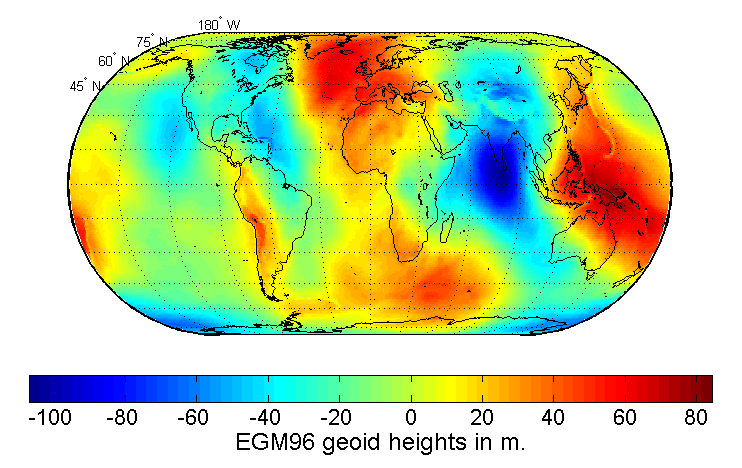
\includegraphics[height=0.22\textheight]{earths_geoidII}
\caption{Difference in meters between the geoid and the ellipsoid \cite{nasageoid}}
\end{figure}

The city of Konstanz, for example, is 46.62 meters above the ellipsoid.

\subsection{WGS84 Coordinates}
A point on Earth's surface is defined by a kartesian coordinate pair consisting of the latitude, that specifies the north-south position and the longitude for the east-west position. 

%IMG

For this work, the degree and decimal fraction representation was selected.

The maximum resolution using 6 fractional digits depends on the position on Earth. In Konstanz, the one degree of longitude equals
% http://en.wikipedia.org/wiki/Longitude#Length_of_a_degree_of_longitude
% lat 11cm
% long 8cm

Google and Apple Maps
The maps images at the closer zoom levels are in most cases taken by a camera mounted on a plane. This camera often does not look perpendicular to the ground but with a gentle angle, so that you can see the building facades.
While this results in a nice isometric-like perspective, it introduces a problem one has to be aware of: Higher parts of the image like higher floors or small hills appear shifted to a certain direction.

%TODO Image

An example: To check the consistency of Google and Apple maps, I initially used the roof window of the office in which the biggest part of this thesis was written. The coordinates of the center of his window on both maps showed a notable discrepancy of several meters. The cause is the different camera angle of the two pictures. 
Measuring the discrepancy using a prominent ground object like the marked lighting, the two map solutions 



\section{Bluetooth Low Energy iBeacons}

Bluetooth Low Energy (BLE) is a standard %TODO year

\section{Swift}

\subsection{What is Swift?}

Swift is a modern programming language released by Apple in 2014. In \cite{swift-book} Apple introduces Swift as "a new programming language for iOS and OS X that builds on the best of C and Objective-C, without the constraints of C compatibility".

Since Swift is a cutting-edge language, this section is dedicated more attention as one would normally do for a implementation language inside a thesis. 

Developers already familiar with the well designed functional programming language Scala will recognize several concepts. It has a concise Syntax avoiding big parts of boilerplate code and syntactic noise, supports functional programming and is statically typed.

The following section is an overview comparison of Scala and Swift features, created during the familiarization with Swift for this thesis. Language features marked will a * will be discussed separately in section \ref{majorDiffs}.

\subsection{Comparison Scala and Swift}

\newcommand{\yes}{yes}

\begin{longtable}{|P{5.5cm}|P{4cm}|P{4cm}|}

\hline \textbf{Language Feature} & \textbf{Scala} & \textbf{Swift} \endhead
\hline Type inference & \yes & \yes \\
\hline Line end separates commands (no need for semicolon) & \yes & \yes\\
\hline Implicit type conversions * & \yes & no \\
\hline Default access levels (access level has to be only provided if it differs from default) & \yes & \yes \\
\hline Functions are first class types\footnote{Functions can be passed to functions, returned from functions, created at runtime and assigned to variables} & \yes & \yes \\
\hline Closures & \yes & \yes \\
\hline Curried functions & \yes & \yes \\
\hline Operator functions & \yes & \yes \\
\hline Named parameters * & \yes & \yes As fixed part of the method's signature \\
\hline Optionals * & via \smalltt{Option[T]} class & widely used, dedicated Syntax\\
\hline Switch with pattern matching & \yes & \yes \\
\hline String interpolation & \yes \newline \smalltt{"Hello \$nameVar"} & \yes \newline \smalltt{"Hello \textbackslash(nameVar)"} \\
\hline Keyword for variable definition & var radius = 1 & var radius = 1 \\
\hline Keyword for constant definition & let pi = 3.14 & val pi = 3.14 \\
\hline Array literal & \smalltt{Array(1,2,3)} & \smalltt{[1,2,3]} \\
\hline Map literal & \smalltt{Map(1->"a", 2->"b")} & \smalltt{[1:"a", 2:"b"]} \footnote{Maps are called dictionaries in Swift} \\
\hline If condition must be boolean & \yes & \yes \\
\hline Tuples & \yes, but without named elements & \yes\\
\hline Ranges & \smalltt{for i <- 0 to 4} \newline \smalltt{0 until 4} & \smalltt{for i in 0...4} \newline \smalltt{0..<4}\\
\hline Constructor & def this() & init() \\
\hline Extended getter/setter concept * & \yes, no observers & \yes, very flexible concept including observers (willSet() didSet() events) \\
\hline Interfaces & trait & protocol \\
\hline Extension of existing types & \yes & \yes \\
\hline Struct & no & \yes \\
\hline Enum & via extending the Enumeration class & \yes, dedicated keyword \\
\hline "Any" Type & Any, AnyVal, AnyRef & Any (instance of any type, even function types) \newline AnyObject (instance of any class type) \\
\hline Qeury an instance of a type by a key in brackets, like arrays or maps & obj(index) calls obj.apply method\newline obj(index) = newValue calls obj.update(0, newValue) & \smalltt{subscript(i:T) -> T2 \{ \newline
\phantom{.} get \{\ldots\} \newline
\phantom{.} set(newValue) \{\ldots\} \newline
\}
} \\
\hline Memory Management & JVM Garbage Collection & Automatic Reference Counting \\
\hline Nested Functions & \yes & \yes \\
\hline Generics & \yes & \yes \\
\hline 

%TODO static

\end{longtable}

\subsection{Major Differences to Scala} \label{majorDiffs}

In this section, the major differences between Scala and Swift that are encountered during the first Swift projects are described.

\subsubsection{Implicit Type Conversions}

In Swift, every type conversion has to be explicit. Even when using different numerical types inside an arithmetic expression, the conversion is not done automatically, in contrast to Scala and even Java. So this code yields a compile time error for example:

\begin{lstlisting}[frame=none]
let a = 1.0
let b = 2
let c = a + b // compiler error: cannot invoke '+' with an argument list of type '(@lvalue Double, @lvalue Int)
\end{lstlisting}

To get an integer 3 assigned to the variable 'c', you need to cast 'a' to Int. For a decimal 3.0, the variable 'b' has to be cast to Double.

\begin{lstlisting}[frame=none]
let c = Int(a) + b    // ok, c is 3 Int
let d = a + Double(b) // ok, d is 3.0 Double
\end{lstlisting}

Although initially it can be a bit frustrating running into compile errors of this kind, you get used to explicitly casting the values to the desired types fast. The advantage of this approach is that the developer explicitly sees the type of the resulting value without having to remember language specific rules.

In contrast, Scala has a powerful implicit type conversion system. Combined with operator overloading it enables developers to create beautiful internal DSL (Domain Specific Languages) that read more like natural language. \footnote{A good example for using implicit conversion to build a DSL query language can be found at \cite{scala-dsl-example}}
But, as M. Odersky rightly wrote in \cite[Chapter 6.13]{scala-book}, "... bear in mind that with power comes responsibility. If used unartfully, both operator methods and implicit conversions can give rise to client code that is hard to read and understand.".

\subsubsection{Optionals}

Variables are non nullable by default in Swift. So the following code will not compile:

\begin{lstlisting}[frame=none, language=swift]
var name = "Swift"
name = nil // compile time error: Type 'String' does not conform to protocol 'NilLiteralConvertible'
\end{lstlisting}

As a consequence, the variable can safely be accessed at any time without the danger of a NullPointerException respectively a nil runtime error.

To allow a variable to assume the value of nil (the null equivalent in Swift), it's type has to be defined as optional by the '?' postfix to the type name.

\begin{lstlisting}[frame=none]
var name:String? = "Swift"
println(name)  // prints 'Optional("Swift")' to the console
println(name!) // prints 'Swift'
name = nil     // ok
let statement = name + " is great" // compile time error: value of optional type 'String?' not unwrapped
println(name!) // runtime error: unexpectedly found nil while unwrapping an Optional value
\end{lstlisting}

The first println statement outputs 'Optional("Swift")' because the string value is wrapped inside the optional and needs to be unwrapped using the '!' postfix. Note that trying to unwrap an optional without value yields a runtime error.

A convenient way of querying properties or calling methods on optionals is called optional chaining. Imagine a circle object with an optional custom style that may have a border, which in turn has an optional custom color. To check the existence of the custom border color, instead of

\begin{lstlisting}[frame=none]
if circle.style != nil && circle.style.border != nil && circle.style.border.color != nil
\end{lstlisting}

it is possible to write

\begin{lstlisting}[frame=none]
if circle.style?.border?.color != nil
\end{lstlisting}

If any link in this chain is nil, the whole chain fails gracefully and returns nil.

Another concept in the context of optionals are failable initializers (known as constructors in other languages). When explicitly defining an initializer as failable appending a question mark (init?), it's return type is optional variant of the type it should initialize. That can be useful for handling invalid parameter values or other initialization problems.

Optionals are widely used in Swift's iOS APIs and their syntax one of the first things noticed when looking to Swift sources as a novice.  
In my opinion, the usage of optionals results in beeing more aware of the presence or absence of values and coding more prudently. Of course, optionals can only add real value if not blindly unwrapped just to silence the compiler errors.  

%TODO cite null pointer ideator

\subsubsection{Getter and Setter}

Swift has a well designed flexible property system, with a concise getter and setter syntax thanks to built-in language support. 

It addresses the two main problems, encapsulation and computing bound to accessing or mutating a property, classical getter and setter methods solve, without the overhead of writing separate accessing and mutating methods for an object's properties.

Encapsulation can be archived by restricting write access to a stored property with the private(set) keyword.

\begin{lstlisting}[frame=none]
private(set) var age = 55
\end{lstlisting}

This restricts write access to the current source file in Swift\footnote{It is still possible to restrict the access to instances of the class by using a separate file for the class definition.}.

In case some computation is needed to update dependent values, Swift offers the willSet and didSet observers that are executed right before and after a stored property is mutated.

\begin{lstlisting}[frame=none]
var age = 55 {
  didSet {
  }
  willSet {
  }
}
\end{lstlisting}

If a property is purely computed, it can be defined in a similar way.

\begin{lstlisting}[frame=none]
var name:String = {
  get {
  }
  set(newName) {
  }
}
\end{lstlisting}

The setter is optional. Nothing changes for the calls for accessing and mutating that property: obj.name = "newName" executes the set block, obj.name the get block.

\subsubsection{Exception Handling}

The exception concept is completely missing in Swift. Unfortunately, there is no official explanation from Swift's designers for this decision.

Using Swift's tuples it is possible to return multiple return values, for example an optional return value paired with an optional error object (cf. \cite{swift-error-handling}):
\begin{lstlisting}[frame=none]
func doSomething(param: String) -> (return: String?, error: NSError?)
\end{lstlisting}

Another option to consider is creating an enumeration with a success and a error member.

\begin{lstlisting}[frame=none]
enum Result {
    case Success(res:Int)
    case Error(msg:String)
}

func next() -> Result {
    return Result.Success(res:3)
}

switch next() {
case .Error(let msg):
    println("Something went wrong: " + msg)
case .Success(let res):
    println("OK: " + String(res))
}\end{lstlisting}

These alternatives misses the exceptions ability to retract some levels of the call stack and retry without explicitly passing an error object up the call chain.
%TODO Erfahrungen Fehlerbehandlung

\subsubsection{Named Parameters}

\subsubsection{The Legacy of Objective-C}

The hardest part of learning a new language is not the grammar itself, but getting familiar with the underlying standard library and special APIs for the myriad of tasks a platform has to be capable to handle nowadays.
Swift uses all the existing Objective-C libraries, which are dynamically translated to Swift using a set of rules to improve the method naming.

For example, Objective-C initializers are mapped to Swift by slicing off the init or initWith part of the first parameter name. So

\begin{lstlisting}[frame=none]
UITableView *myTableView = [[UITableView alloc] initWithFrame:CGRectZero style:UITableViewStyleGrouped];
\end{lstlisting}
becomes
\begin{lstlisting}[frame=none]
let myTableView: UITableView = UITableView(frame: CGRectZero, style: .Grouped)
\end{lstlisting}
in Swift (cf. \cite{swift-objc-book}).

For several tasks it is necessary to mark an own class or protocol with the "@objc" attribute\footnote{Attributes are the counterpart of annotations in the Java world.}, that makes it available in Objective-C code. 

An example: Objective-C APIs sometimes use selectors, which are strings identifying a certain callback method by its method name and its named parameters that will be called on the passed object.
When an API is used that expects a selector as parameter, the @objc attribute is needed on the passed object's class, so that that the library can find and call the method, otherwise at runtime a fatal error occurs stating no method with that name can be found.
This is a clear limitation of that automatic translation of old APIs. In my opinion, it would be much safer to rewrite this APIs in Swift and replace all selectors with function parameters or closures. This way, a misspelled method name is recognized at compile time.

Because of the usage of old Objective-C standard libraries, learning Swift automatically means - at least to a certain degree - learning Objective-C, too. 

\subsubsection{Summary}

Swift is currently the most modern programming language available for any mobile platform. Although it's expressive and concise syntax and it's Playground and REPL (Read-Eval-Print-Loop) feature, Swift remains a compiled language. Like Objective C, it is compiled into machine code by the LLVM compiler, which proved to be very fast. Being a new language, the tooling is not yet very stable.\footnote{At the time of writing, the XCode IDE doesn't support any refactoring in swift. The compiler isn't fully finished (a few language elements cause a "Not yet implemented" error), some error messages are cryptic and misleading, the context assistance doesn't always work and the editor can get stuck after some editing with phantom errors that are hard to remove.}

Despite of the problems in this early stage, Swift is - in my opinion - a great Language and a big step forward compared with it's predecessor Objective C. It will likely become even better as time passes and the language and tooling matures. 


%TODO Parallel execution

\section{iOS and Cocoa Touch}

iOS Cocoa Touch Framework 
Developing with XCode

\section{Couchbase NoSQL Database}


\subsection{What is a NoSQL Database?}

For a long time, designing the persistence layer of a system meant deciding which relational database to use. Former alternative approaches like object oriented databases failed to establish themselves. 
However, during the last few years, more and more companies and projects are rely on a new kind of database system: NoSQL.

Unfortunately, no precise definition exists for a NoSQL database system. In their Book "NoSQL Distilled" \cite{nosqldistilled}, which provides a good and concise introduction to NoSQL, P. Sadalage and M. Fowler try to provide five common characteristics of NoSQL databases:

\begin{itemize}
\item Not using the relational model
\item Running well on clusters
\item Open-source
\item Built for the 21st century web estates
\item Schemaless
\end{itemize}

As they emphasize in their book, they think relational databases will not disappear. But the innovation is seeing relational databases as an option among others, and choosing the one that best fits a project.\footnote{Sometimes that even means choosing different database types for several parts of a single system - what is called polyglot persistence.} 

\subsection{Couchbase}

Couchbase\cite{Internet-couchbase} is a modern JSON-based NoSQL database, available as an open-source community edition used in this thesis. While JSON was initially born as "Javascript Object Notation" for data exchange between web / application servers and the javascript web gui, today it is used in more and more products independently from javascript. It's simplicity, readability and compactness helped to repress the comparatively cumbersome XML in many areas. Especially document-oriented databases like Couchbase use the JSON notation for storing the structured data of it's documents.

Couchbase offers a specially sleek mobile version - called "Couchbase Mobile" or "Couchbase Lite" - for all major mobile platforms, and so of course for iOS, too. Since especially mobile devices cannot rely on an uninterrupted networking connection, the mobile version a good choice for a network independent local cache of the application data. With it's synchronization functionality, the local mobile database can be automatically synchronized with a database server. Every time a network connection is available, the local database is updated with changes on the server, and local changes made during the offline time are propagated to the server.

To connect the mobile version to a regular Couchbase server, a sync gateway has to be set up:

\begin{figure}[H]
\centering
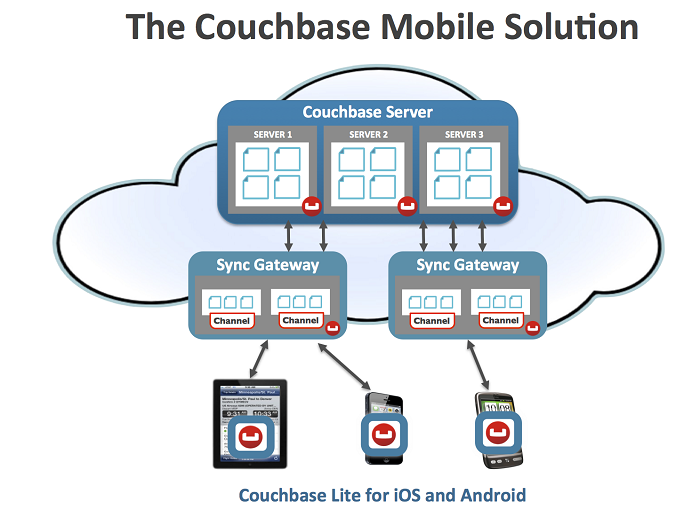
\includegraphics[height=0.25\textheight]{couchbase-lite}
\caption{Couchbase Lite and Sync Gateways. From \cite{couchbase-lite}}
\end{figure}

While traditional relational database management systems (RDBMS) are typically hard to scale out\footnote{also "Horizontal Scaling" - dividing a database over several servers after reaching the limit of upgrading a single server with more powerful hardware (vertical scaling)}, Couchbase offers a built-in distributed cache concept that can easily be scaled on more servers without modifying the application.

Queries are performed using the map reduce programming model originally developed by Google Engineers, allowing massive parallel execution (cf. \cite{MapReduceArticle}). This enables couchbase to perform computation and storage heavy big data analytics.

Couchbase was chosen for this work for it's mobile variant, it's synchronization abilities over several databases and it's JSON-based documents that are a good fit for the web back end and are easy to read and create manually.


\section{Typesafe Reactive Platform}

\subsection{Overview}

In 2013, Typesafe Inc. launched the "Reactive Manifesto", that was updated in September 2014 to the Version 2.0 \cite{reactivemanifesto}. The core message is as follows: "We believe that a coherent approach to systems architecture is needed, and we believe that all necessary aspects are already recognised individually: we want systems that are Responsive, Resilient, Elastic and Message Driven. We call these Reactive Systems."

The Typesafe Reactive Platform consists of the Play web framework, the Akka message driven runtime and the Scala programming language. It focuses on providing the tools needed to build highly responsive applications, that not only are easy to scale, but even able to increase and decrease the allocated resources at runtime to handle varying workload (thus be "elastic") and stay responsive even in case of failure (what is called to be "resilient").

Since it's publication, the manifesto and the platform gained rising attention. In my opinion, this platform has a high potential of getting the de facto standard of how modern software systems are developed during the next decade.

The Typesafe Reactive Platform is used in this thesis for building the backend part of the system, as Scala application with a Play web gui and an NoSQL Couchbase driver based on Akka, that will be introduced later. %TODO in Chapter xy

\subsection{Activator Tool}

Typesafe Activator is a dependency manager and build tool for the reactive platform built upon sbt (Simple Build Tool, sometimes Scala Build Tool). So it completely replaces sbt, understanding all commands formerly issued to sbt. In the Play framework, it replaces the Play command, which also was a wrapper around sbt. (cf. \cite{typesafeact}). It comes with an optional browser based ui for quickly creating some sample projects and an inspection feature for monitoring Play requests and akka actors. 

\subsection{Play Web Framework}


The Play Web Framework v1.0 was released on 19th October 2009. For version 2.0, released in March 2012, it was completely rewritten in Scala.
Although inspired by popular high-productivity web frameworks like Ruby on Rails or Groovy on Grails, it comes with full type safety typical for Scala but missed in the other frameworks.

Play is a full-stack web framework.

\begin{figure}[H]
\centering
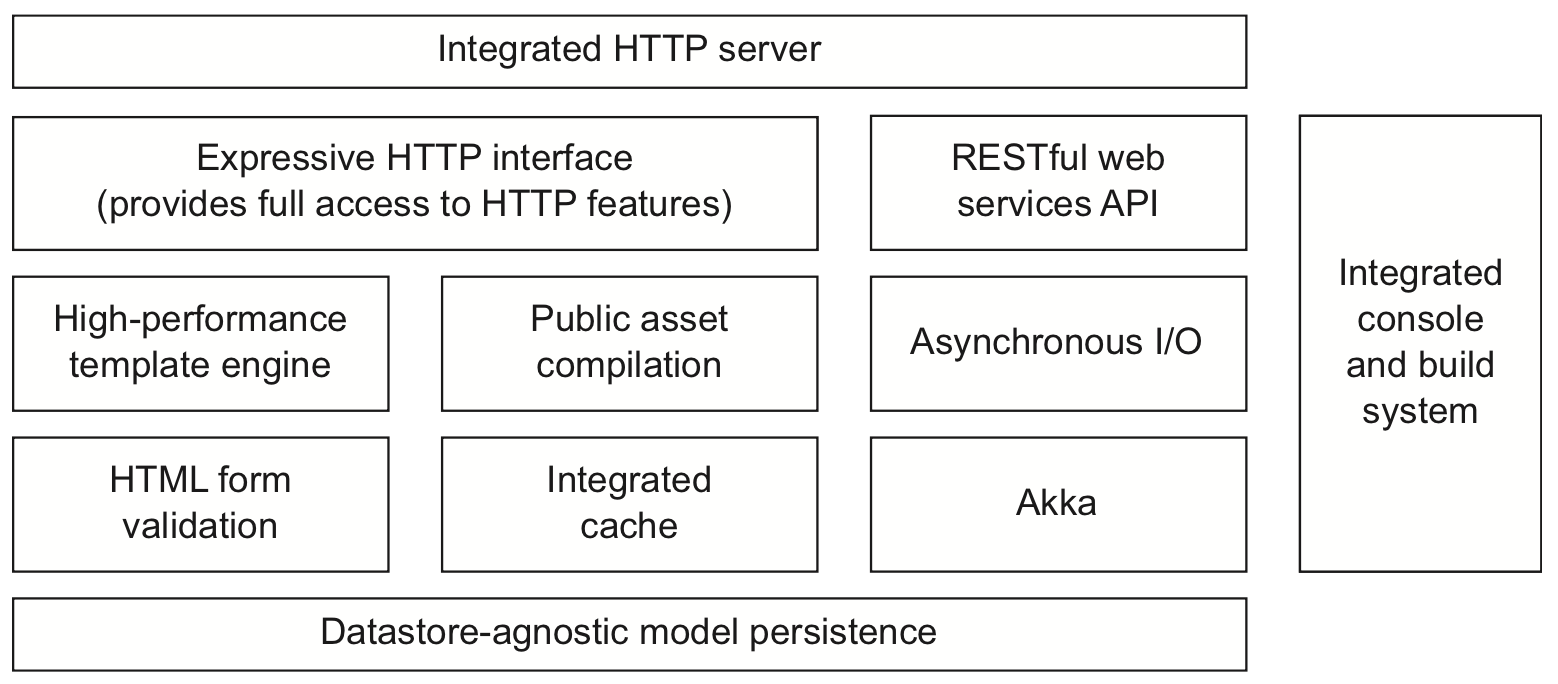
\includegraphics[height=0.25\textheight]{play-stack}
\caption{The Play framework stack. From \cite{play-book}.}
\end{figure}

The key features that make Play are:
 
\begin{itemize}
\item Integrated HTTP Server ("JBoss Netty")
\item RESTful web services API 
\item Type-safe templates for defining the html user interface
\item Central mapping from HTTP requests, including type-safe parameters, to the corresponding Scala controller method
\item Integrated build system that automatically rebuilds when the page is reloaded in the browser.
\item Ability to test the web application without a browser or even a running web server and call controller methods or render templates directly from a Scala REPL with the pre-loaded project 
\item Support for AJAX, Comet and WebSockets
%TODO
\end{itemize} 
% Chapter 3

\chapter{System Overview} % Main chapter title

\label{systemoverview} % For referencing the chapter elsewhere, use \ref{Chapter1} 

\lhead{Chapter 3. \emph{System Overview}} % This is for the header on each page - perhaps a shortened title

%----------------------------------------------------------------------------------------

\section{Introduction}

The Context-Aware Guide (subsequently called "CA Guide") needs to be defined to fit indoor and outdoor exhibitions, like classical museums, parks and gardens. 
The basic functionality must be accessible even by persons not familiar with mobile technology. The context awareness techniques can help avoid big parts of explicit user input.

The following figure shows an overview of the complete system, consisting of a museum guide front-end running on a mobile device, a back-end for the configuration of the guide and performing analytic functions. A database server is accessed by both system parts and represents the communication basis - there is no direct communication between font and back end. All data is exchanged over the database, enabling asynchronous communication.

As database server Couchbase was choosen due to it's automatic synchronization capabilities, it's mobile version and it's ability to scale out without completely redesigning the way the database is accessed by the application.\footnote{After actually having reached the limits of scalabity of a single classical relational database server of a commercial project and painfully distributing the database on several servers of the productive system, the idea of an easy scale out using a document based database and map-reduce queries seemed even more ingenious to me.} 

\begin{figure}[H]
\centering
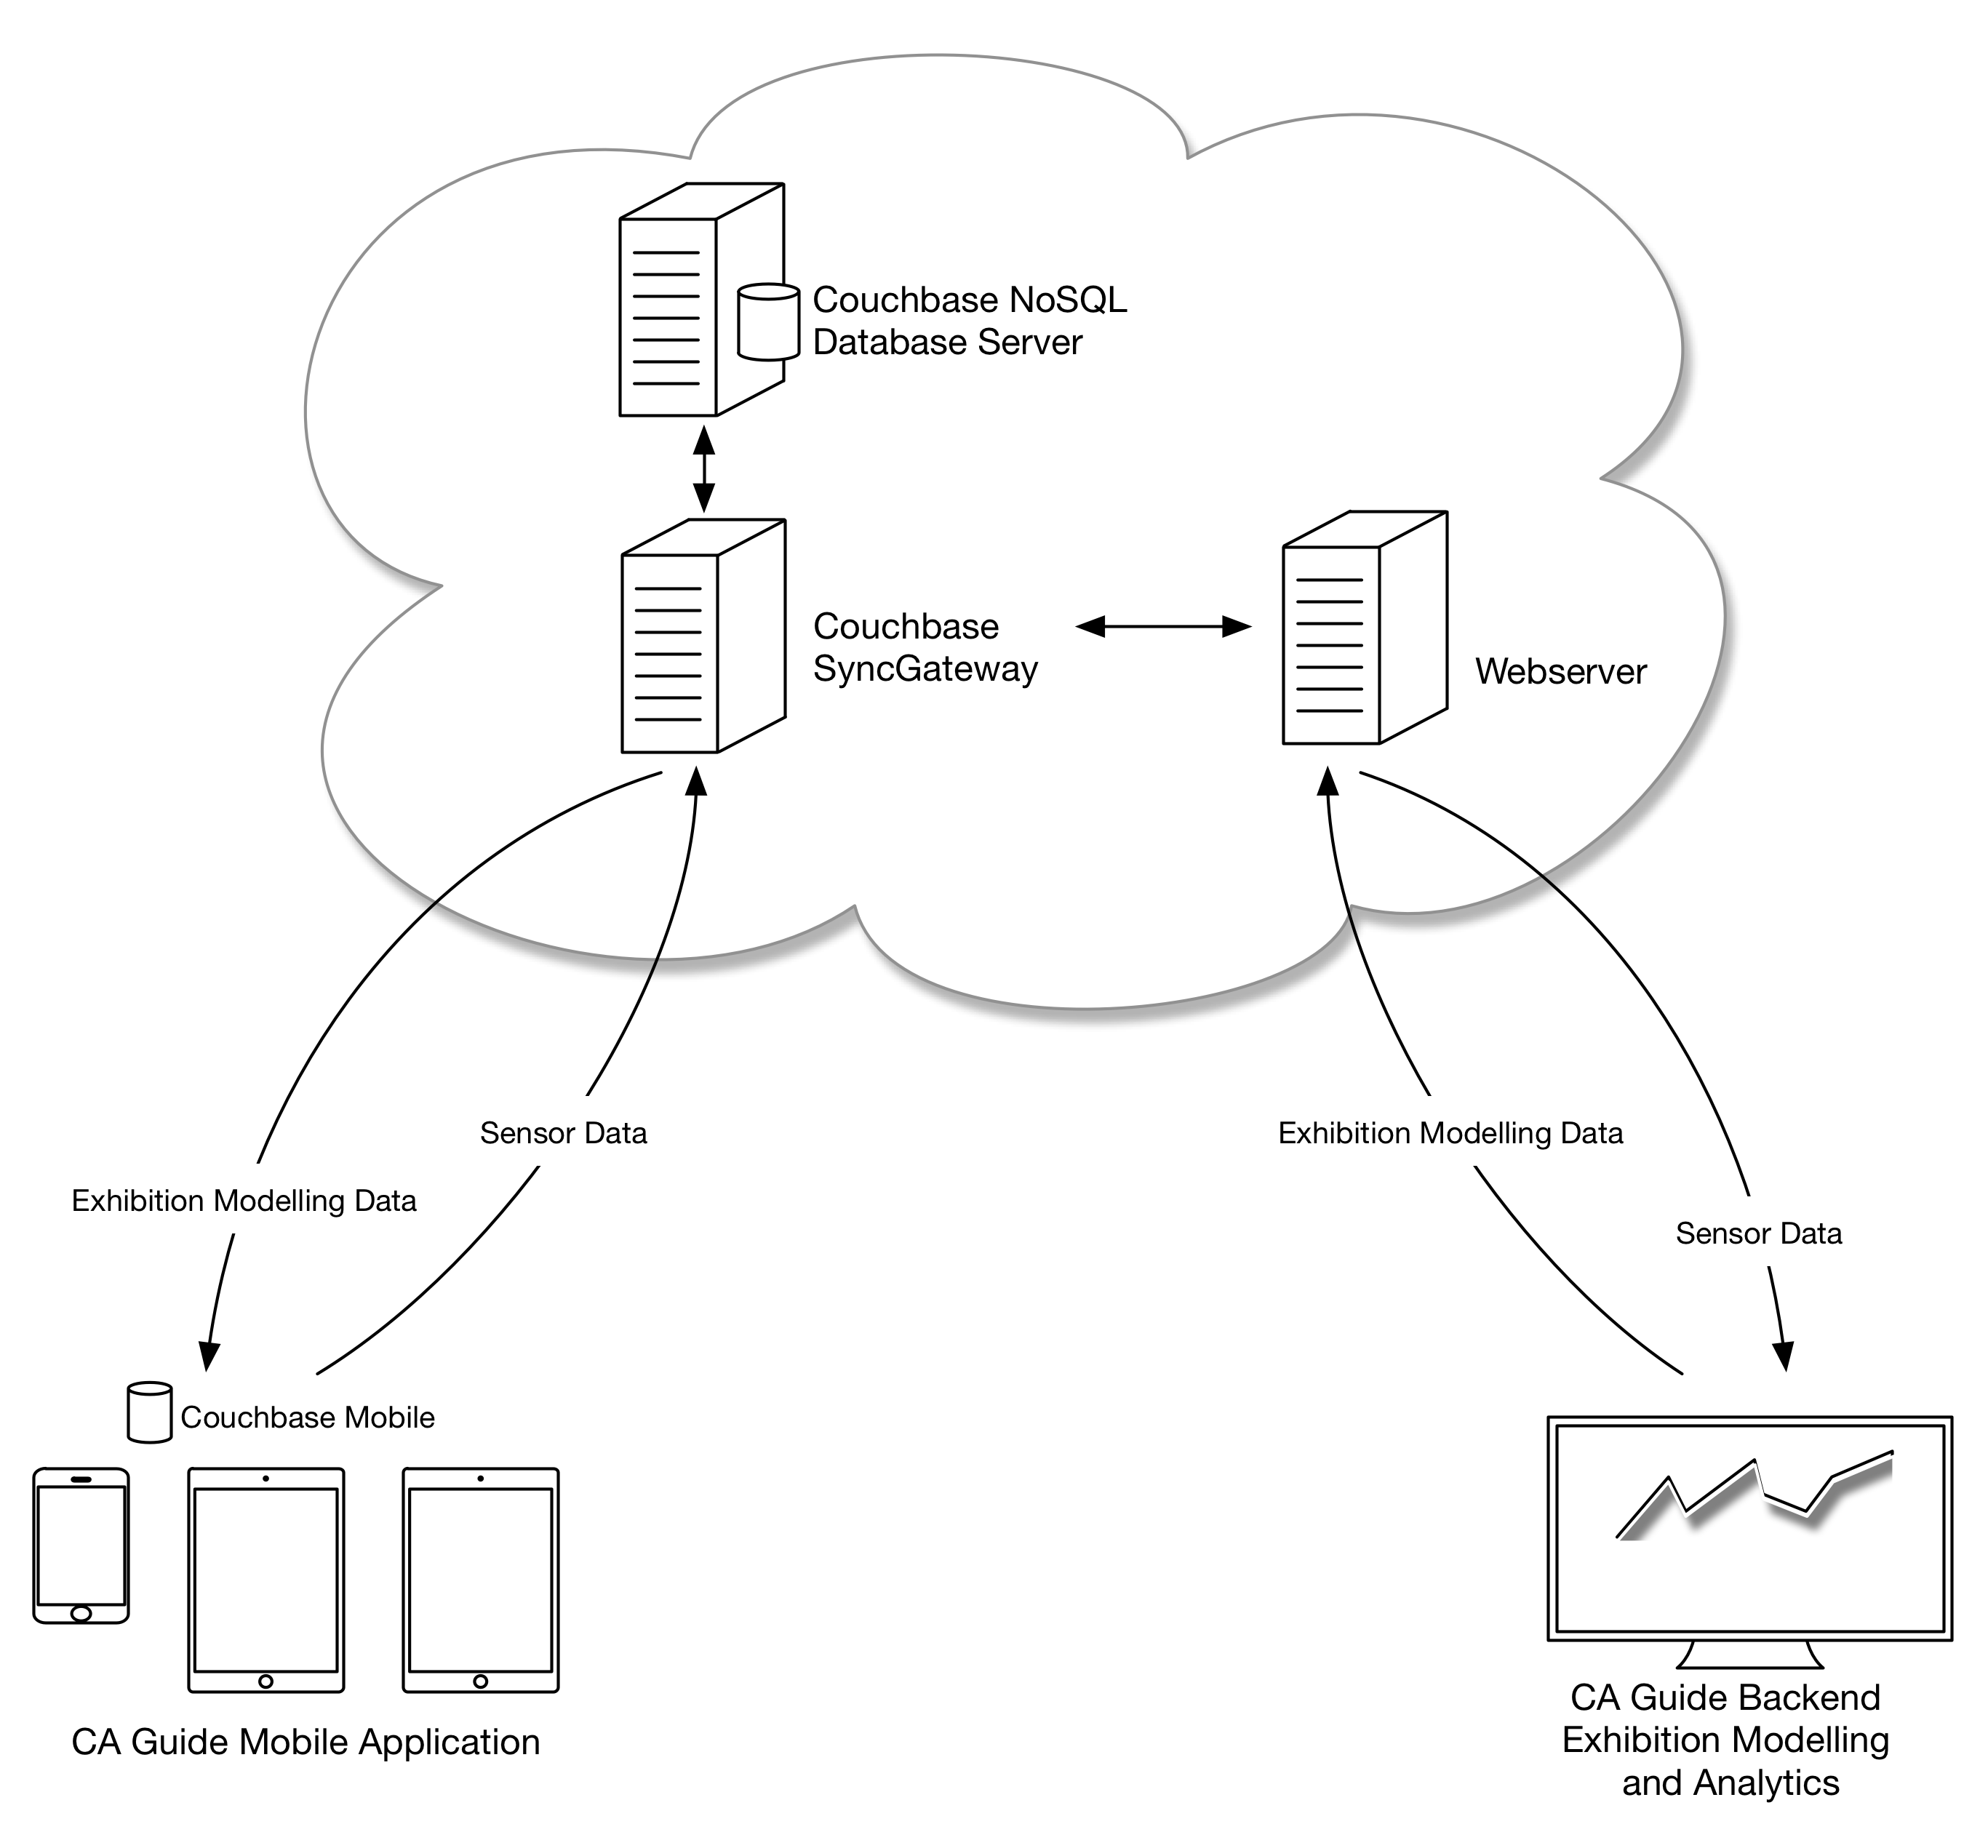
\includegraphics[height=0.8\textwidth]{system-overview}
\caption{CA Guite Architecture Overview}
\end{figure}

Image Mockup CA Guide 

Image A Backend Screen Mockup

\section{Data Structure}

\subsection{Exhibition Modelling}

A single exhibition is modeled in the JSON data format. Compared to XML, JSON is more readable and easier to produce without dedicated tools in a simple text editor.

The entities needed for modelling an exhibition are:

Image entyty relationship diagram

With a normal relational database, pretty much of the entities would be saved in separate tables using primary keys and foreign keys to represent the relationships between the tables.

In a document-oriented database the whole exhibition can be stored in an aggregated way. 

\begin{lstlisting}
key: "exhibition-CXN01"
value: {
 "type":"exhibition",
 "city":"Konstanz",
 "pois": [{
	 "name":"Dom", 
	 "locationDefinition": {
	 	"type": "circle",
	 	"location": [15.0020312,2.3434322],
	 	"radius": 30,
	 	"floor": 1
	 }, 
	 "text":"", 
	 "images":[], 
	 "audio":{
	 	"level1":
	 	"level2":
	 	"level3":
	 }, 
	 "videos":[]},]
}
\end{lstlisting}

A JSON Schema is used for asserting a valid structure of a JSON file, similar to a DTD (Data Type Definition) in XML (http://json-schema.org).

\subsection{Sensor Data}

Sensor data is saved to the Couchbase database to allow replaying it for development, testing, presentations and for analytics presented in the system's web backend. 

The single measurements can be very high frequent, for example in case of accelerometer data, that is updated every 10 millisecons. New beacon measurements are available every second. Events on a higher logical level, like "entering region a", will occur less frequently.

\begin{lstlisting}[basicstyle=\footnotesize]
key: SENSORTRACE-CXN01
value: {
  "date": "2015-02-12",
  "time": "20:15",
  "accelerometer": [
    {"timestamp": 12345678.35, "data": [1.235, 0.364, 0.021]},
    {"timestamp": 12345678.40, "data": [1.217, 0.378, 0.009]},
    ...
  ],
  "gyroscope": [
    {"timestamp": 12345678.35, "data": [1.235, 0.364, 0.021]},
    {"timestamp": 12345678.40, "data": [1.217, 0.378, 0.009]},
    ...
  ],
  "magnetometer": [
    {"timestamp": 12345678.35, "data": [1.235, 0.364, 0.021]},
    {"timestamp": 12345678.40, "data": [1.217, 0.378, 0.009]},
    ...
  ],
  "beacons": [
    {"timestamp": 12345679.05, "data": [["A3F3", -51],["85B7", -68]]},
    {"timestamp": 12345680.05, "data": [["A3F3", -51],["85B7", -68]]},
    ...
  ],
  "gps": [
    {"timestamp": 12345679.35, "data": [1.44, 10.021]},
    {"timestamp": 12345680.36, "data": [1.44, 10.009]},
    ...
  ],
}
\end{lstlisting}


\section{Setting up the Couchbase Infrastructure}

Couchbase Server
Admin Port

Couchbase Sync Gateway
config.json
% Chapter 4

\chapter{CA Guide Frontend} % Main chapter title

\label{frontend} % For referencing the chapter elsewhere, use \ref{Chapter1} 

\lhead{Chapter 4. \emph{Museum Guide Frontend}} % This is for the header on each page - perhaps a shortened title

%----------------------------------------------------------------------------------------

\section{Architecture}

A fundamental requirement for the CA Guide frontend, the mobile application, is the ability to automatically test the single layers using recorded sensor data and comparing it with it's expected result.

To achieve this level of testability, virtual sensors are introduced at three different levels of abstraction:
 
\begin{figure}[H]
\centering
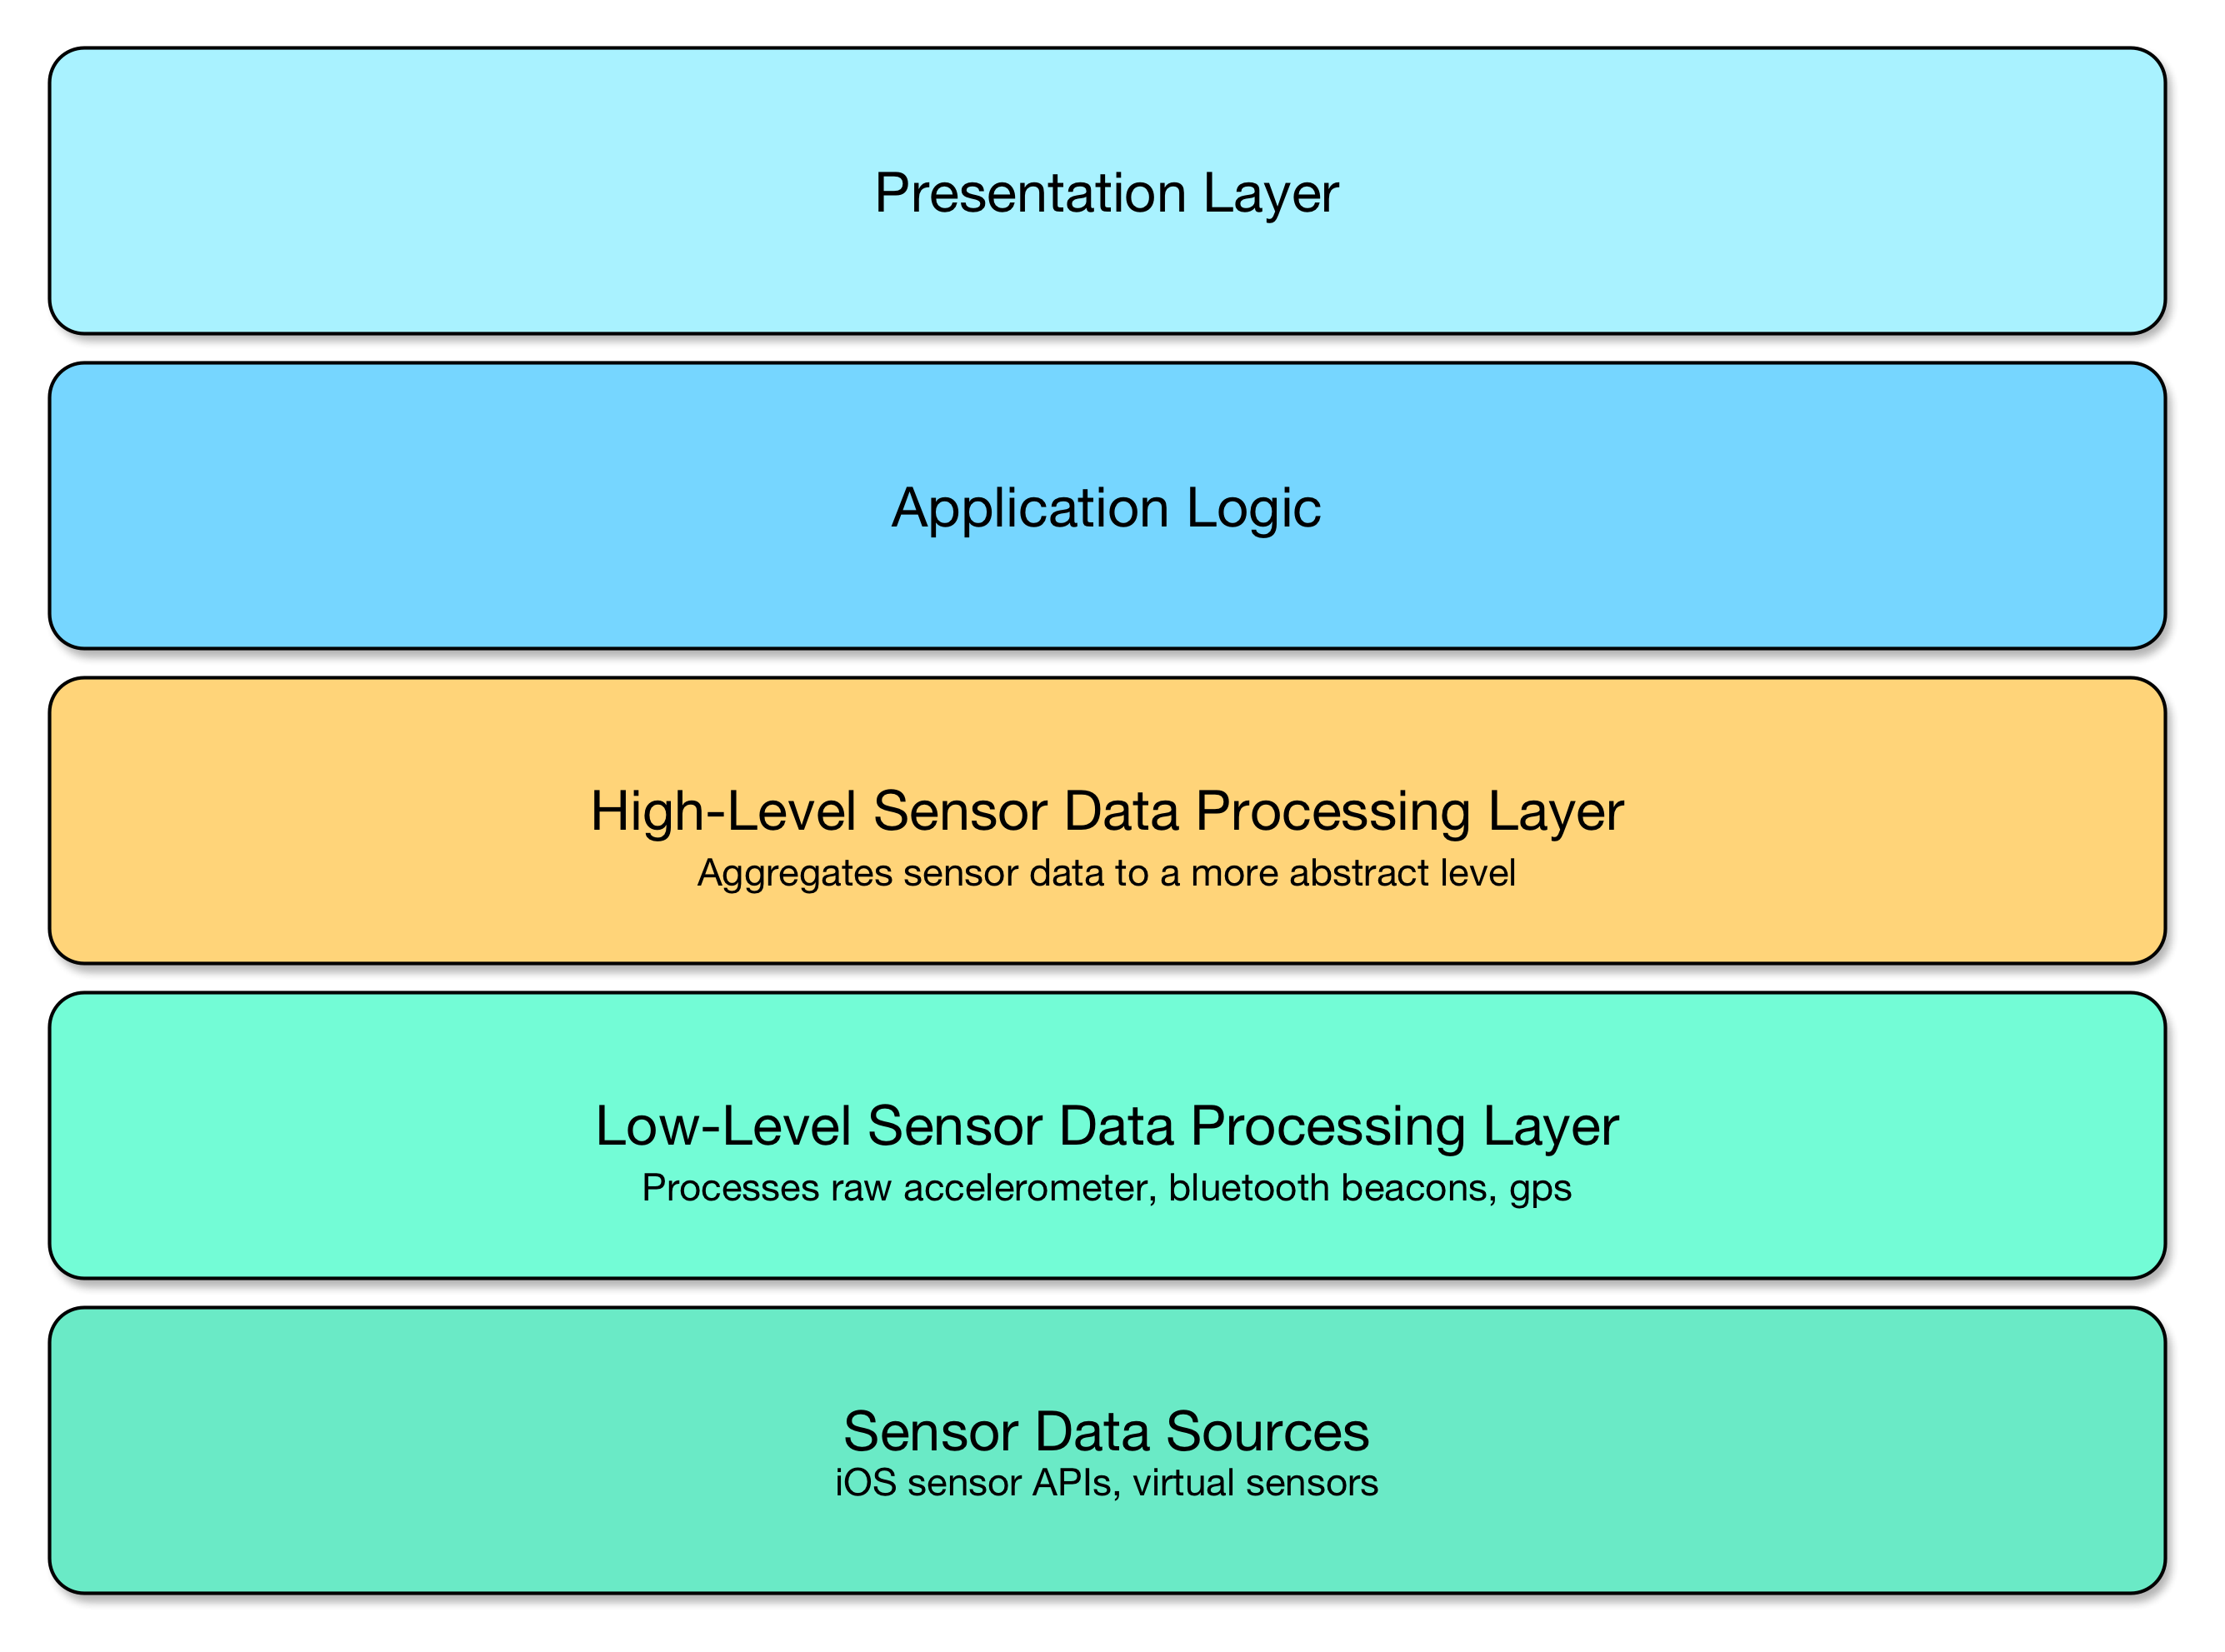
\includegraphics[width=0.9\textwidth]{layers-guide-app.png}
\caption{Layer Model of the Museum Guide Application}
\end{figure}

\begin{figure}[H]
\centering
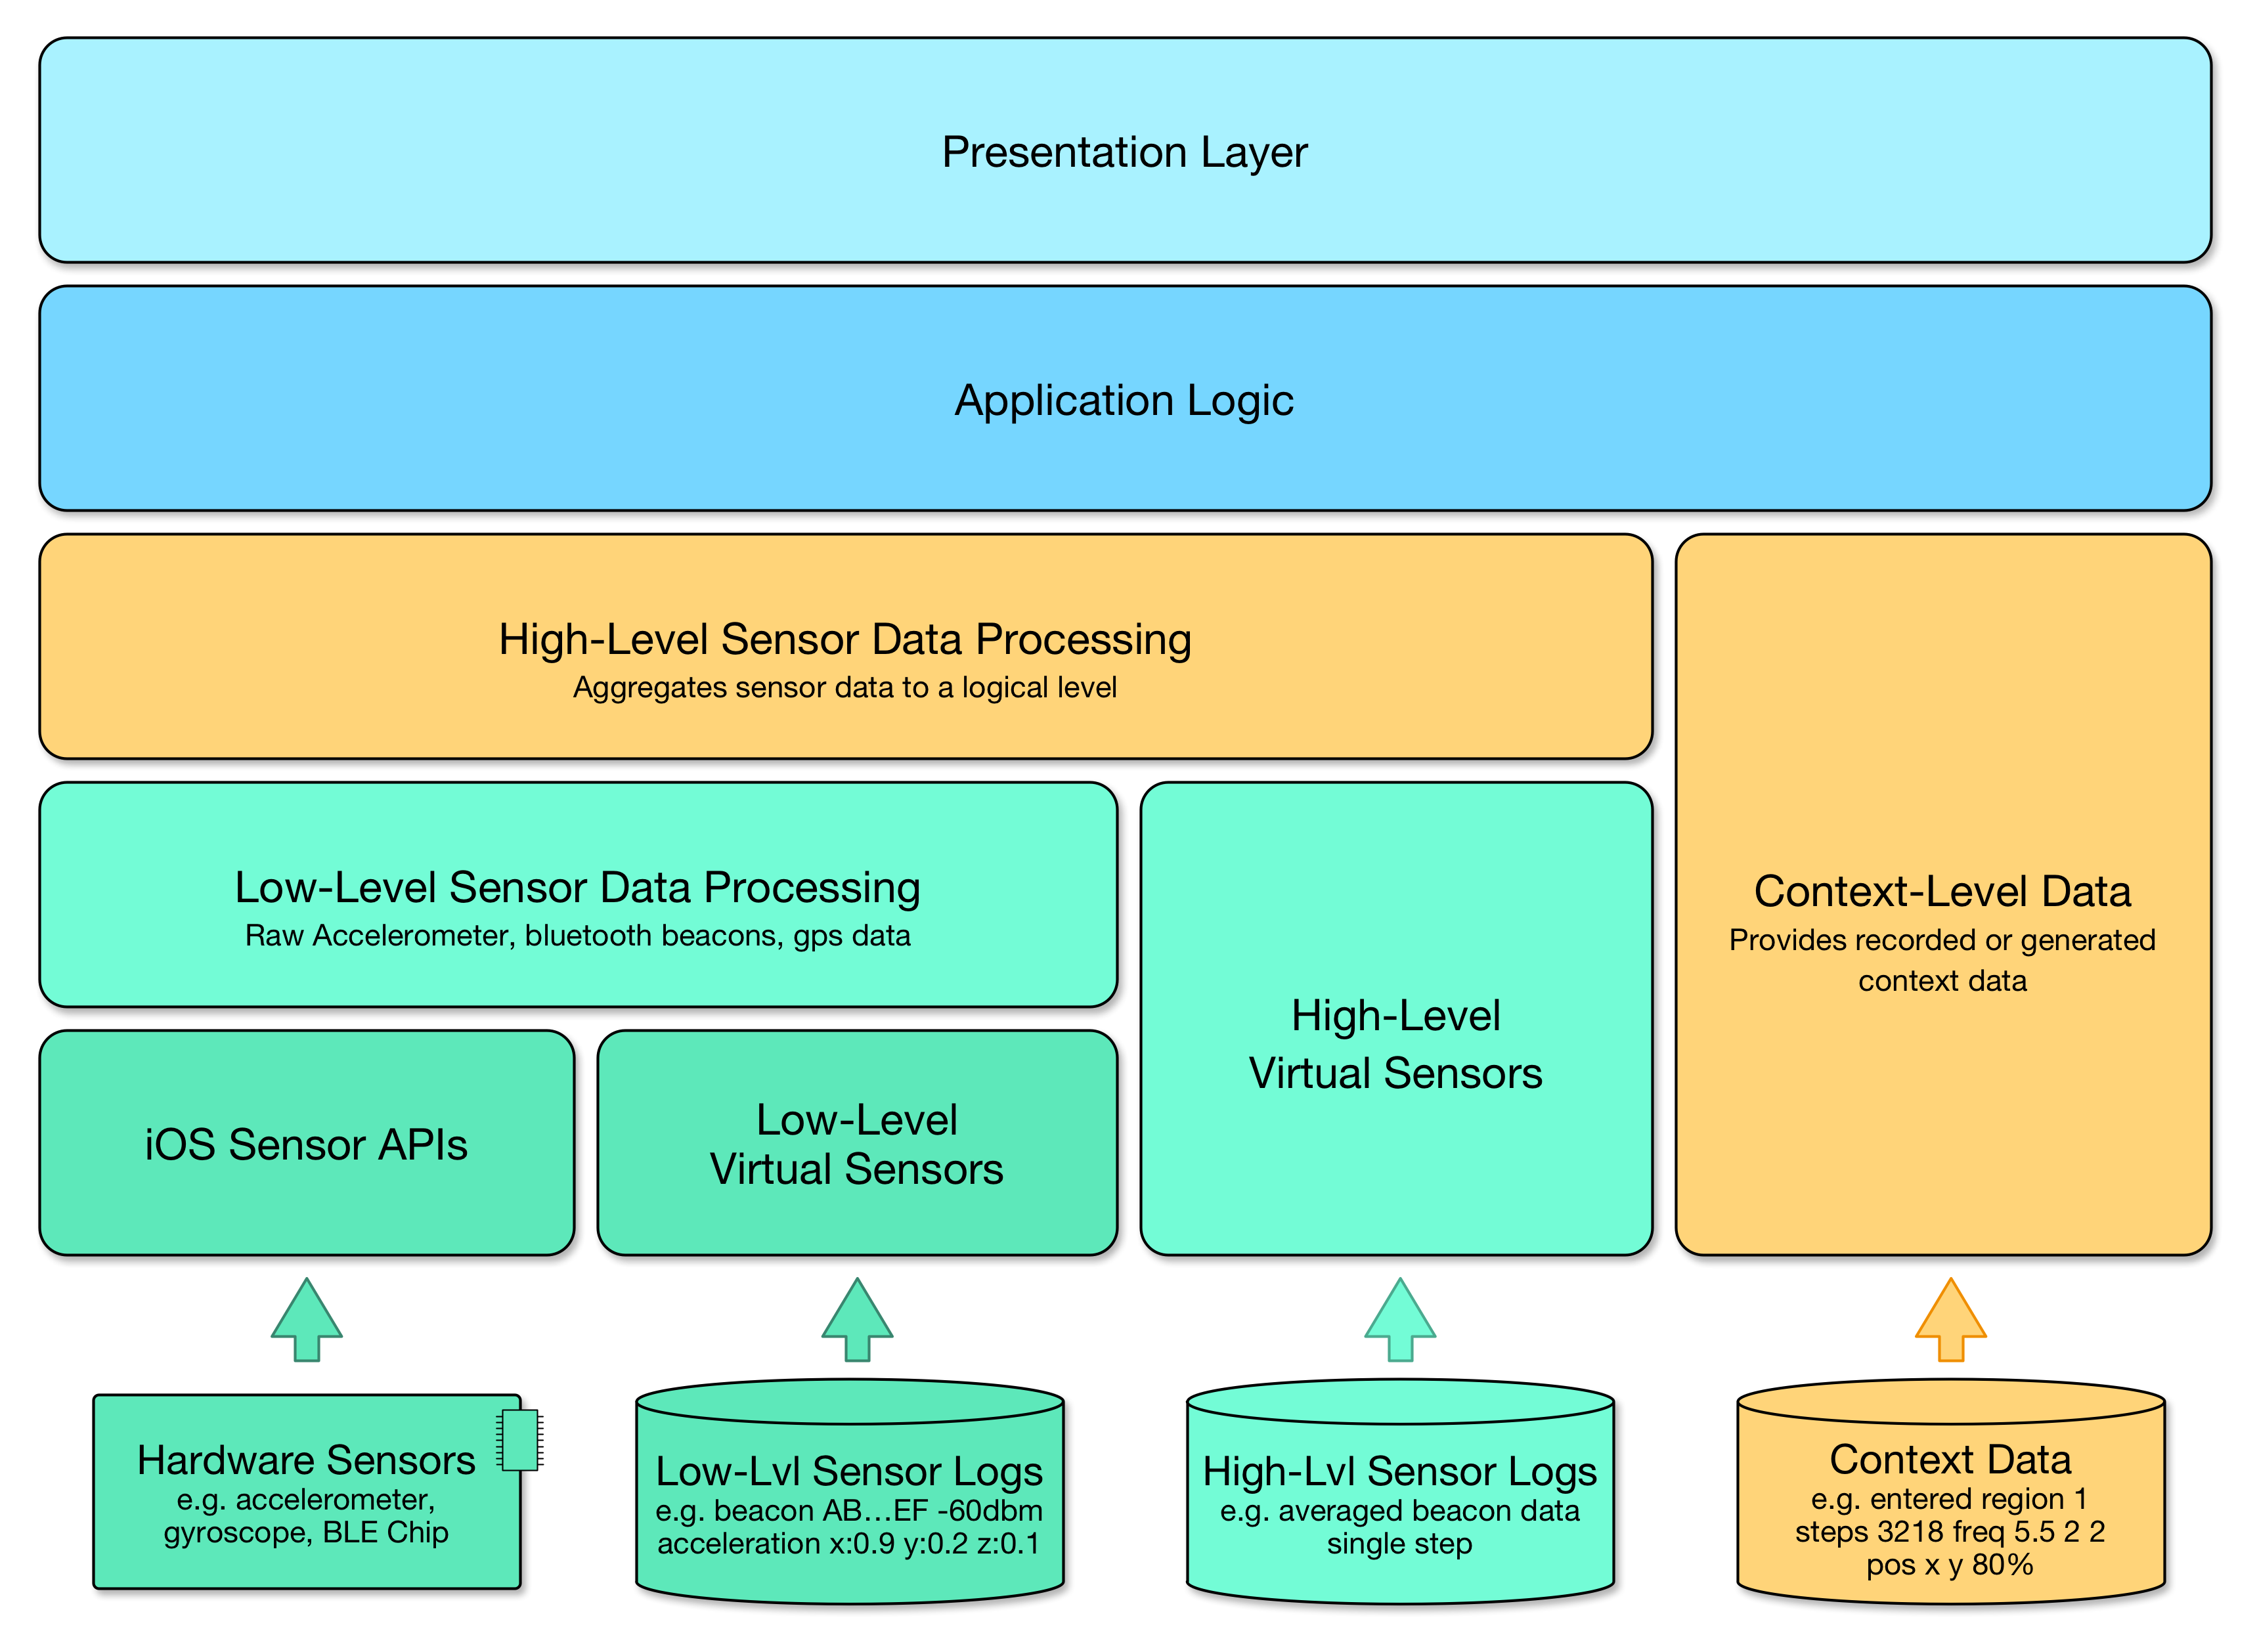
\includegraphics[width=0.9\textwidth]{layers-guide-refined-app.png}
\caption{Refined Layer Model}
\end{figure}

Virtual sensors of different levels for 
development 
automated testing
presentations  
easier migration to a different platform

\begin{figure}[H]
\centering
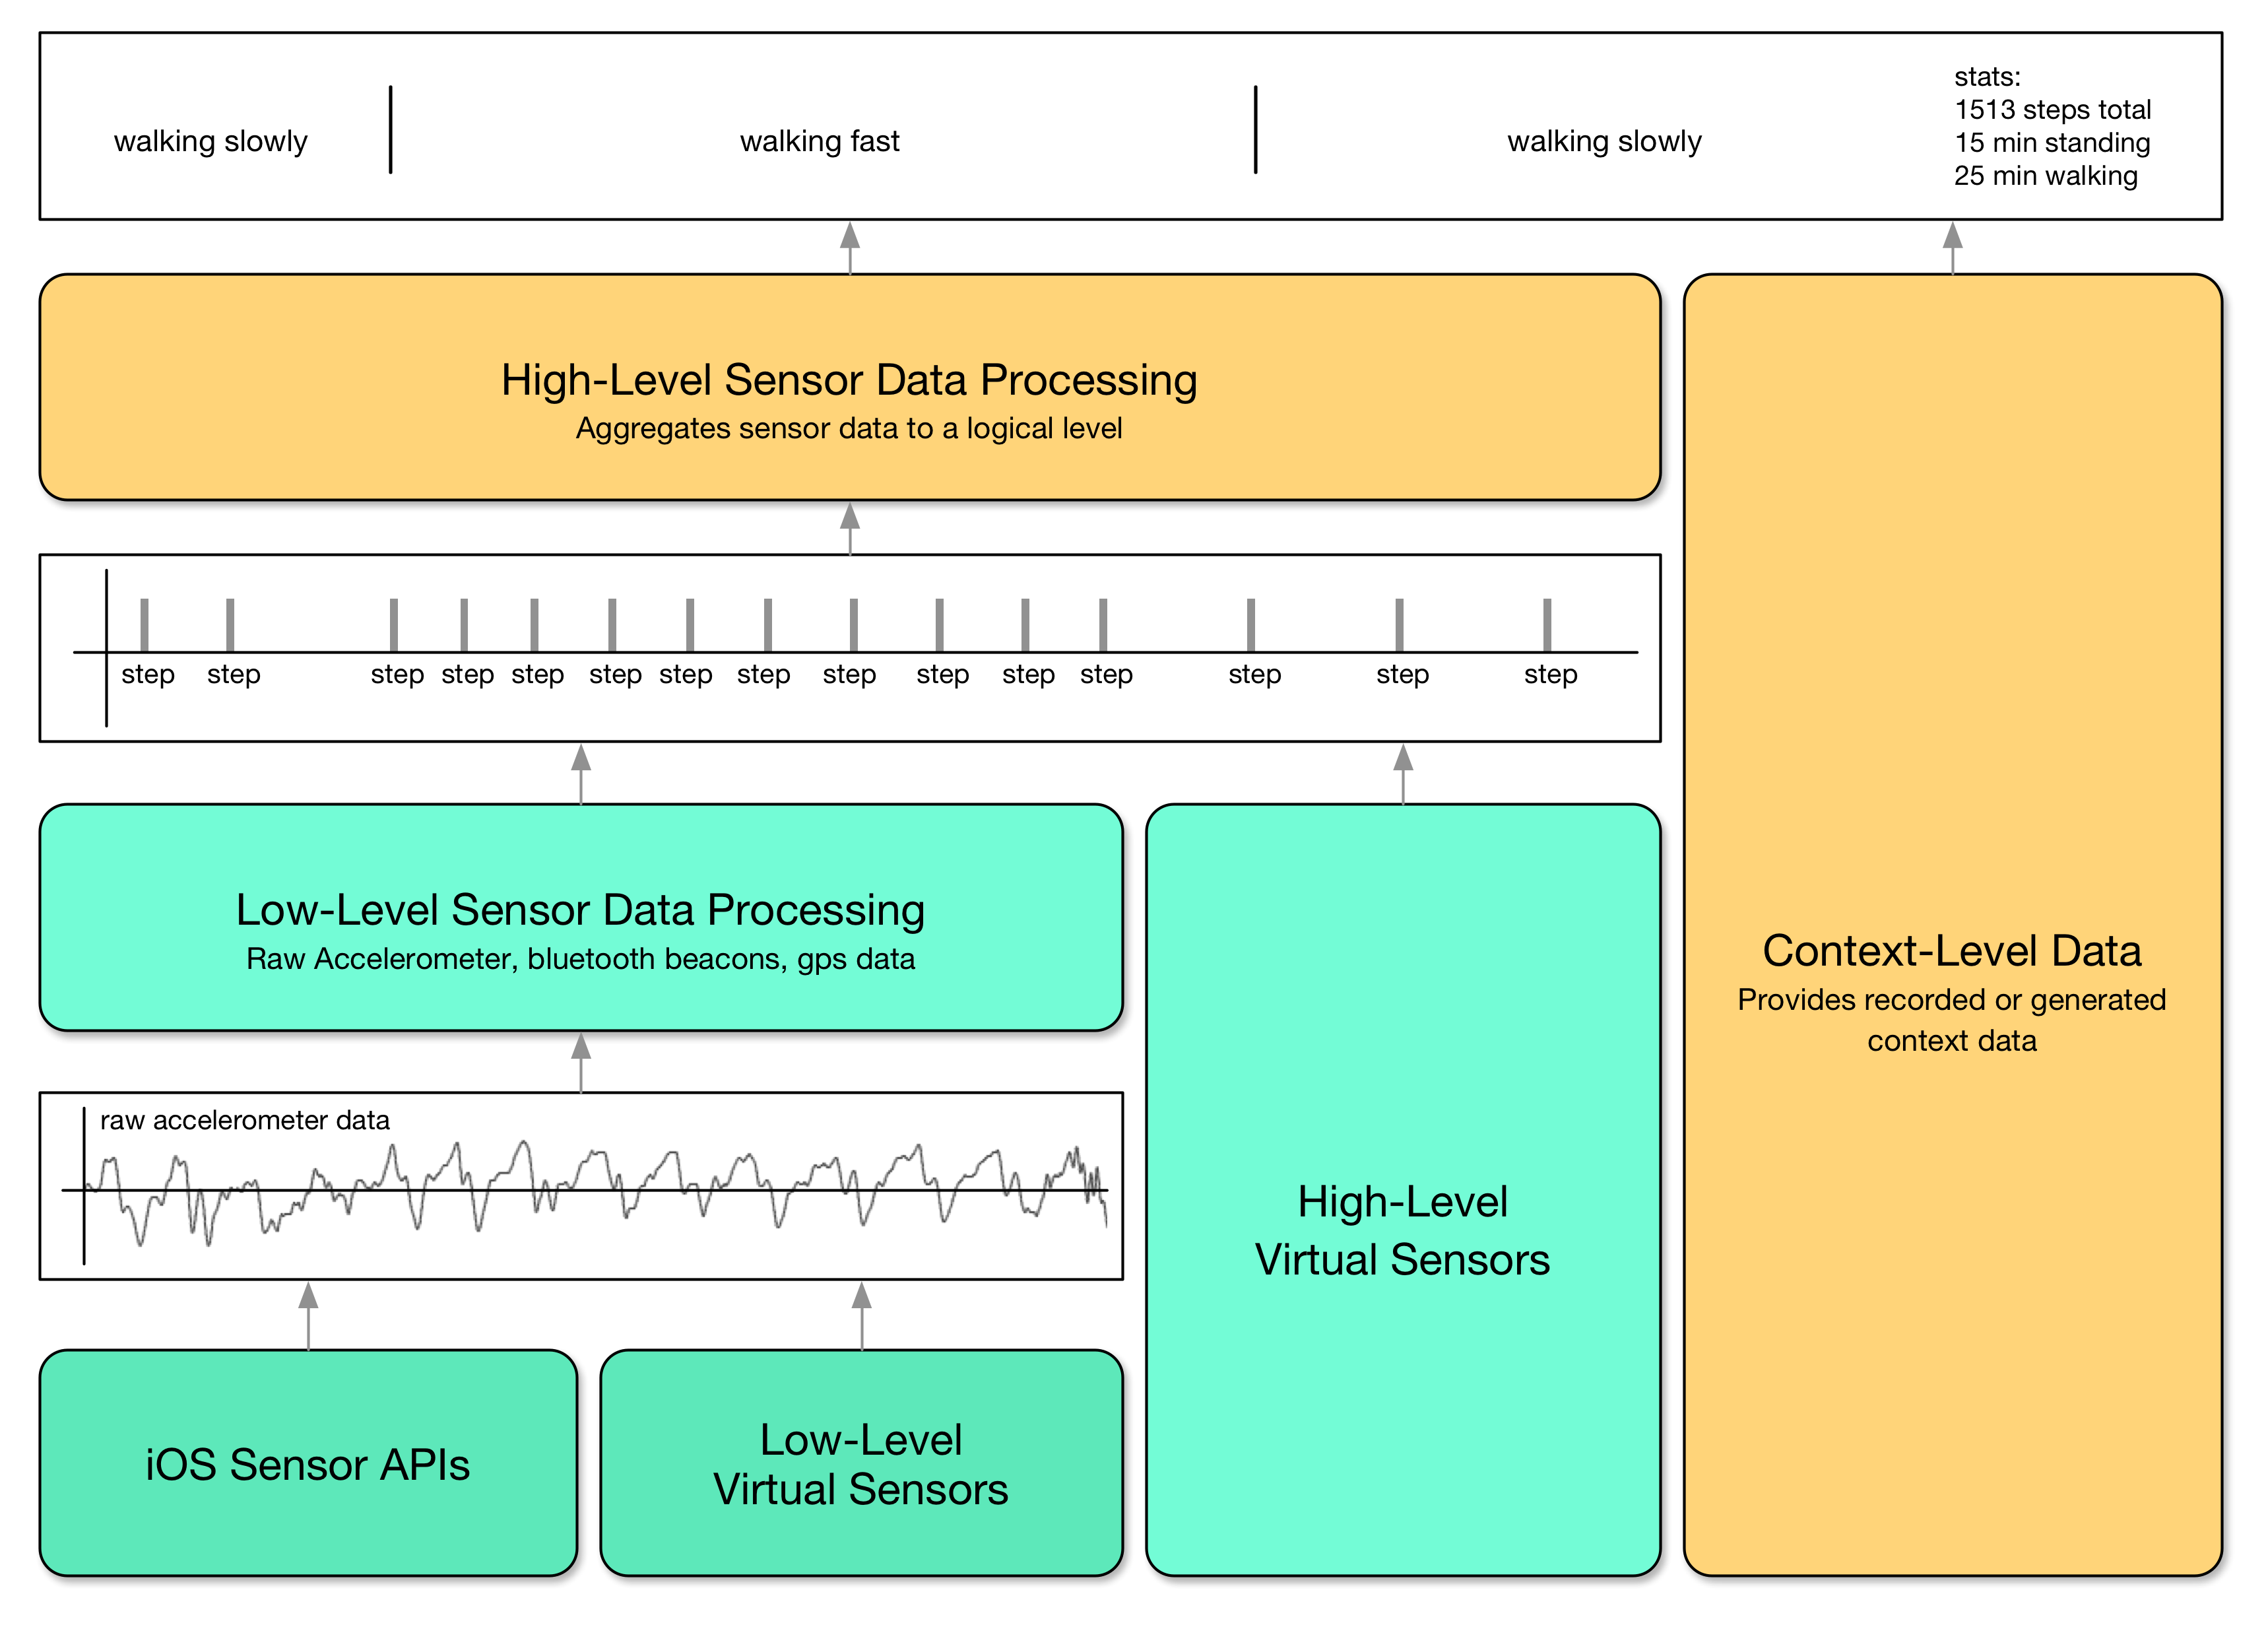
\includegraphics[width=0.9\textwidth]{layers-app-dataflow-accelerometer.png}
\caption{Data Flow between the lower Layers}
\end{figure}

Real Time Data

\begin{figure}[H]
\centering
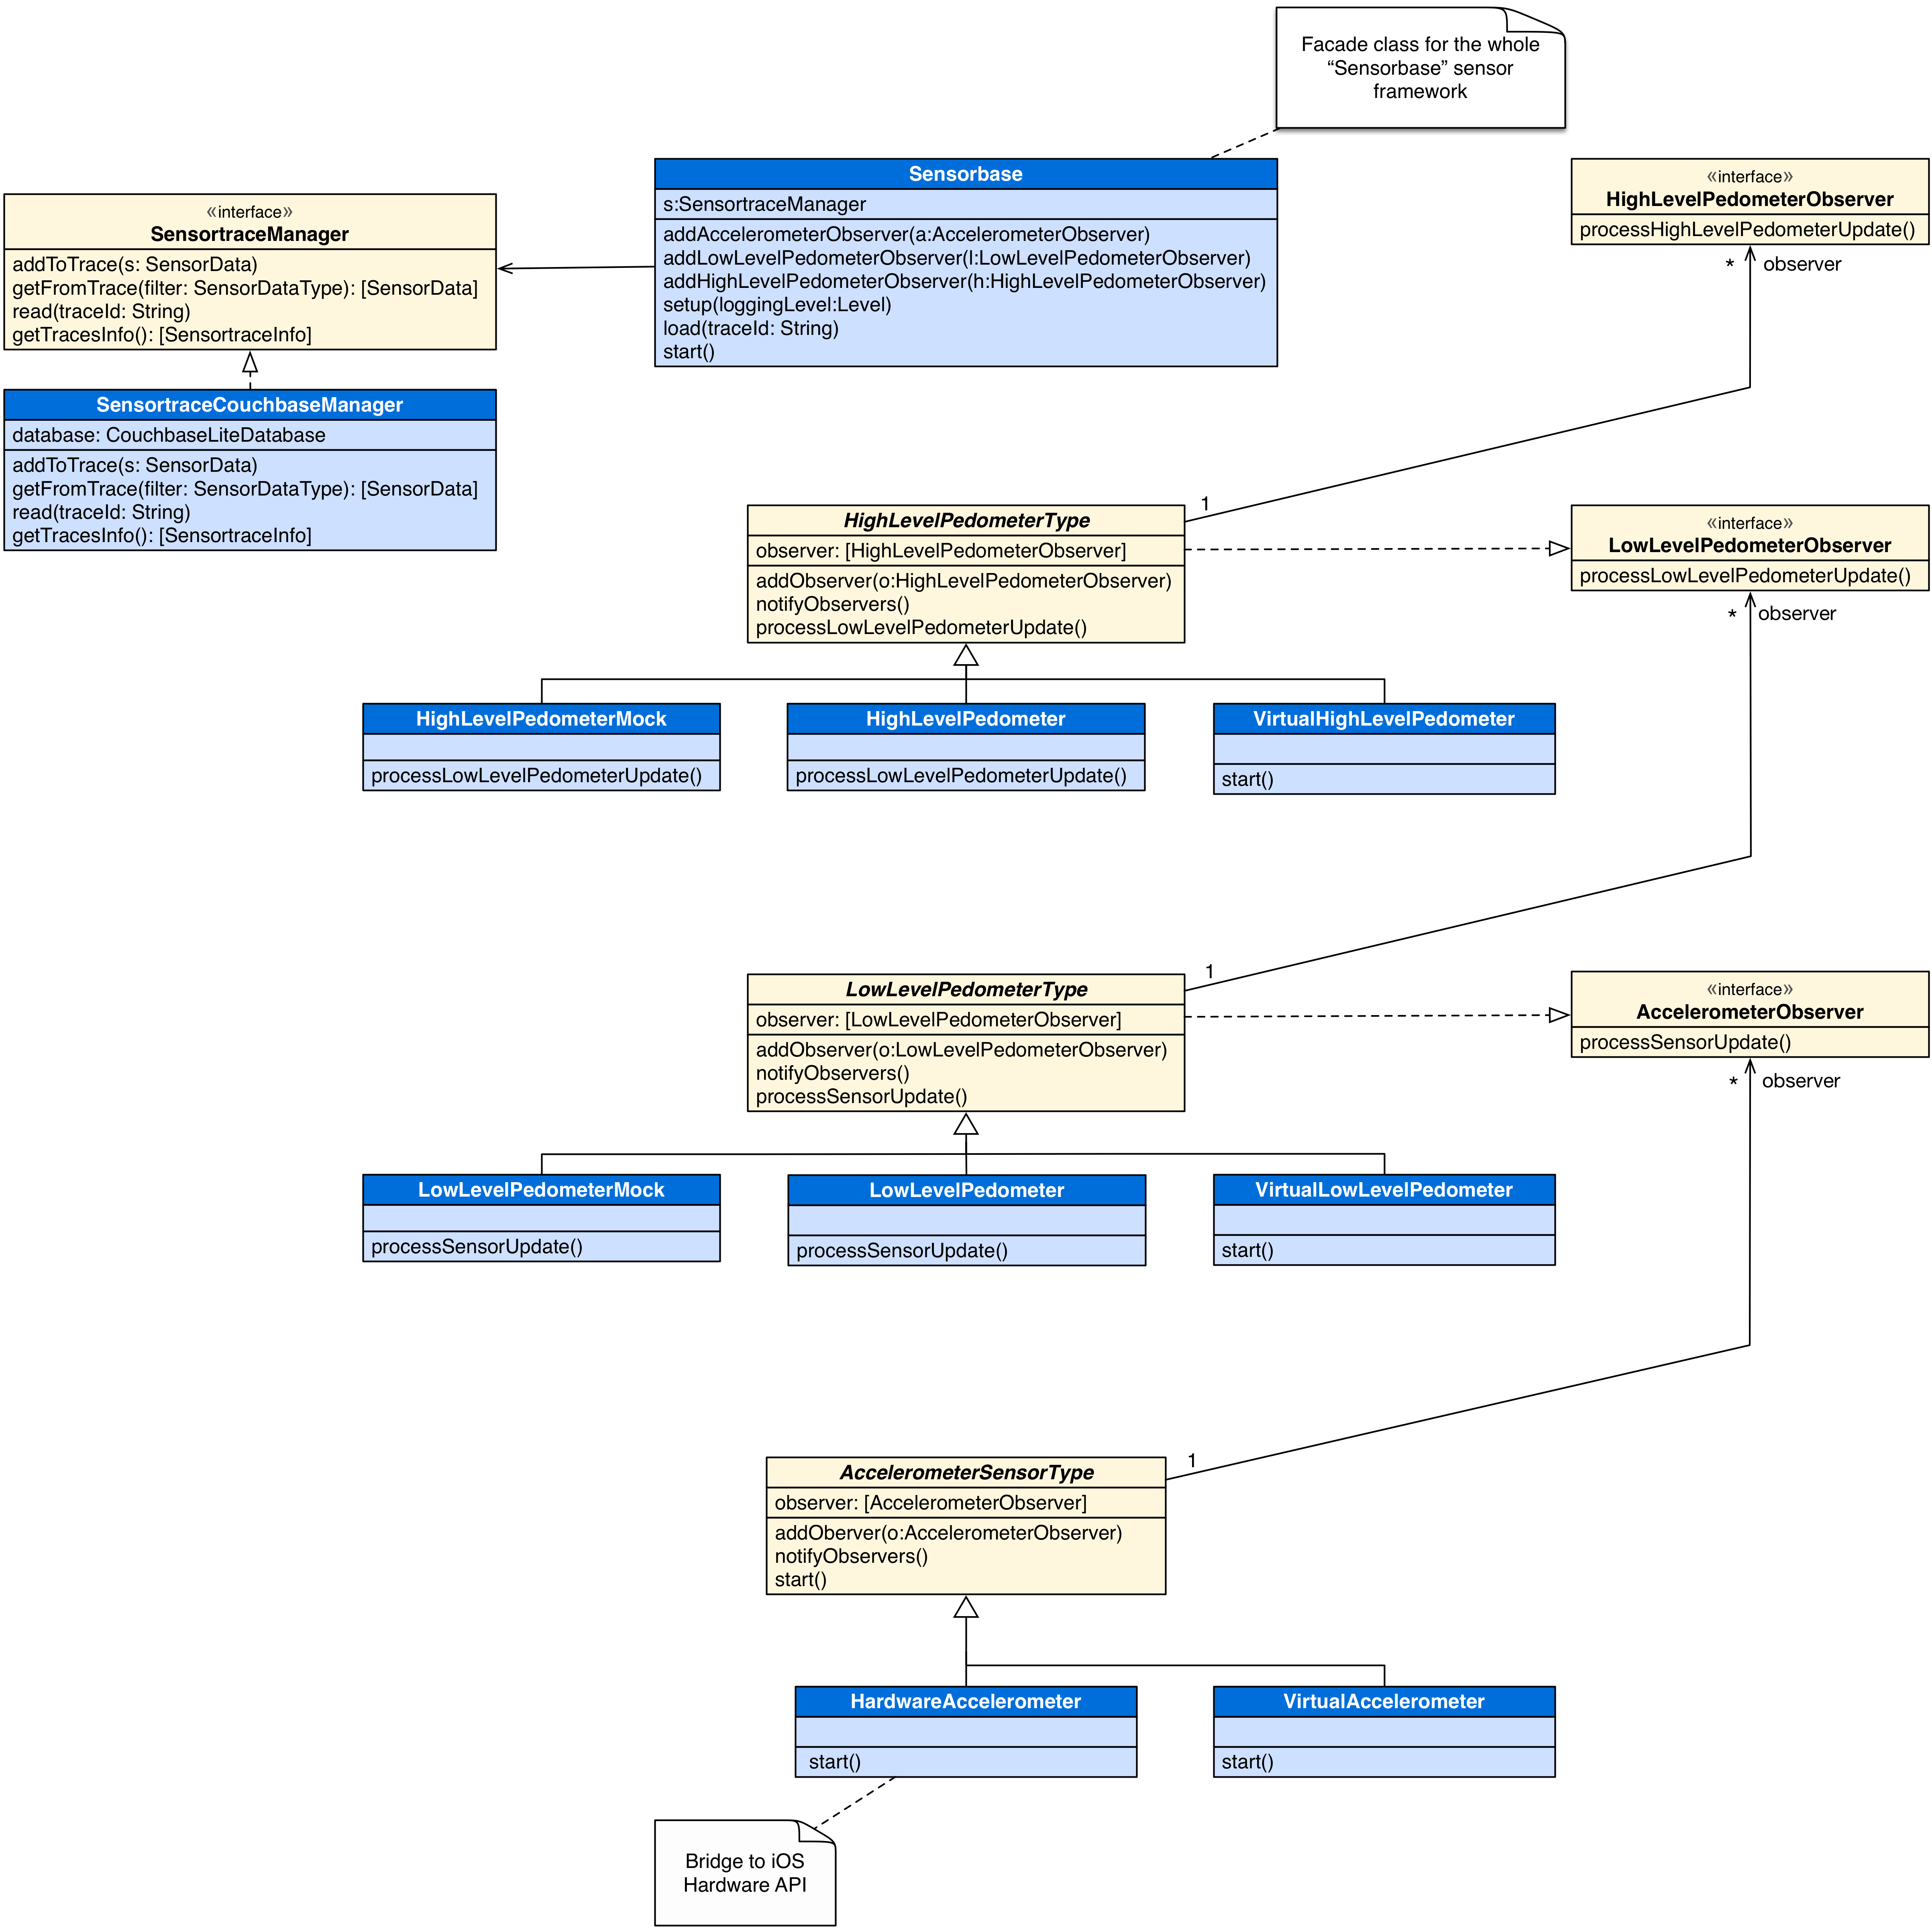
\includegraphics[width=1.0\textwidth]{class-diagram-guide-app.png}
\caption{Simplified Class Diagram for Sensor Data Processing}
\end{figure}

Mock: useful for Testing the underlying layer,
Adapter


\section{Sensors Layers}

Sensor data is saved to couchbase database.
Later access for replay (development), testing and presentations.
The backend can access this saved data for later analysis.

\section{Application Logic}

If not walking fast load and play current content.

If display is on show actions that user has to opt in, if display is off play automatically. 

\section{Presentation Layer}

Mockups
XCode Storyboard
Final App Screenshots
% Chapter 5

\chapter{CA Guide Back End} % Main chapter title

\label{backend} % For referencing the chapter elsewhere, use \ref{Chapter1} 

\lhead{Chapter 5. \emph{CA Guide Back End}} % This is for the header on each page - perhaps a shortened title

%----------------------------------------------------------------------------------------

\section{Introduction}

The CA Guide back end is meant to be used by the park or museum staff responsible for designing and optimizing the visiting experience. In contrast to the front end, the user interface can be more complex requiring an introductory training and support. Of course, the usability deserves special attention in spite of the training, as it has a major influence on the frequency a software is used, the attitude towards it and so the success of the whole product. %TODO Citation

There are two main tasks accomplished with the CA Guide back end:

\begin{itemize}
\item Modeling the outdoor or indoor site by defining areas on a map or floor plan and adding content that later will be presented on the mobile device when entering this area. Especially for indoor sites, single Bluetooth beacons with their identifying numbers and positions must be added to the plan to enable the mobile device to locate itself.
\item Analytic functions for understanding how the visitors move trough the exhibition and thus allowing to optimize it, similar to the way the behavior of website visitors is tracked and used to optimize the web presence\footnote{Of course, the privacy of the visitor has to be respected at any time. The data must only be collected anonymously and respecting all local privacy and data protection regulations.}.
\end{itemize}

%TODO In Place editing

\section{The Target Platform}

The back end user interface has to run in a standard web browser without specific plugins. This has several advantages: Users can start immediately to work with the product without installing any client. Having the project data in a cloud database, they can work on the same project from different locations using different computers without manually setting up a synchronization infrastructure. Computation expensive analytic functions can be performed directly on the database or web/application servers and only the results are transferred to the client, enabling it's usage on common hardware.

By allowing collaborative editing, the museum staff can easily be supported remotely in real time without having to be on site. 

\section{Architectural Decisions}

\subsection{The Client and Server Code Gap}
One of the main challenges developing for the web is the client/server code barrier. 

Modern web applications need to be highly responsive for providing a good user experience and thus be accepted by them. Operations like adding, editing or deleting entities have to be performed without having to do a full page reload to display some sort of HTML form and reloading the whole page again after the form was submitted to the server. This can be achieved using asynchronous calls to the server in the background, exchanging only the needed data with the server and refreshing just the needed part of the HTML DOM. Many operations like resorting a table can even be performed completely in the browser without even performing a server request.

This technique is commonly known as AJAX (Asynchronuous JavaScript and XML) and inside this acronym's phrase one can already spot the main problem. While AJAX gained popularity during the last years, it leveraged the massive usage of JavaScript, a dynamically typed scripting language originally not designed for big projects. In fact, JavaScript\footnote{In the cited interview Eich says "The name is a total lie" - it was just a marketing decision. JavaScript has been standardized later by Ecma International to ECMAScript.} was developed in 1995 by Brendan Eich in ten days for the Netscape browser, which is an extremely short time despite Eich's big experience in building languages \cite{interview-eich}. That led him to design the language to be malleable, and there are many libraries making programming in JavaScript a little "less painful", without solving the problem of lacking static types and other flaws.

So the two main problems to be solved are:

\begin{itemize}
\item Some data structures and algorithms already existing in the server code have to reprogrammed for the client running in the browser, creating redundancy with all the known problems it has
\item The standard programming language for client-side code lacks static typing and a class syntax, among others
\end{itemize}

The next subsection focuses on different solution attempts.

\subsection{Solution Attempts}

\subsubsection{Improved Javascript}

In the last years, several new scripting languages are emerging that compile to JavaScript. 

One of this languages was even integrated in the Play framework, which comes with an built in compiler for CoffeeScript \cite{coffeescript}. It is a small language that provides a nicer syntax for JavaScript, introducing even classes and inheritance, and compiles to plain JavaScript. However, it does not add any support for static typing.

Another noteworthy web-client language is TypeScript, which is maintained by Microsoft as open source \cite{typescript}. As the name implies, it adds static typing to JavaScript with type inference and similar to CoffeeScript it enhances the syntax. In contrast to CoffeeScript, it is a superset of JavaScript, meaning any JavaScript code is automatically valid TypeScript code, too. 
For using third party libraries in a typed way, a big repository with open source type definitions for 796 libraries at the time of writing \cite{typescript-repo}. By including a reference to such a type definition, the library's API can be accessed in a statically typed way.

This screenshot demonstrates a TypeScript compilation error and an inferred numeric type.
\begin{figure}[H]
\centering
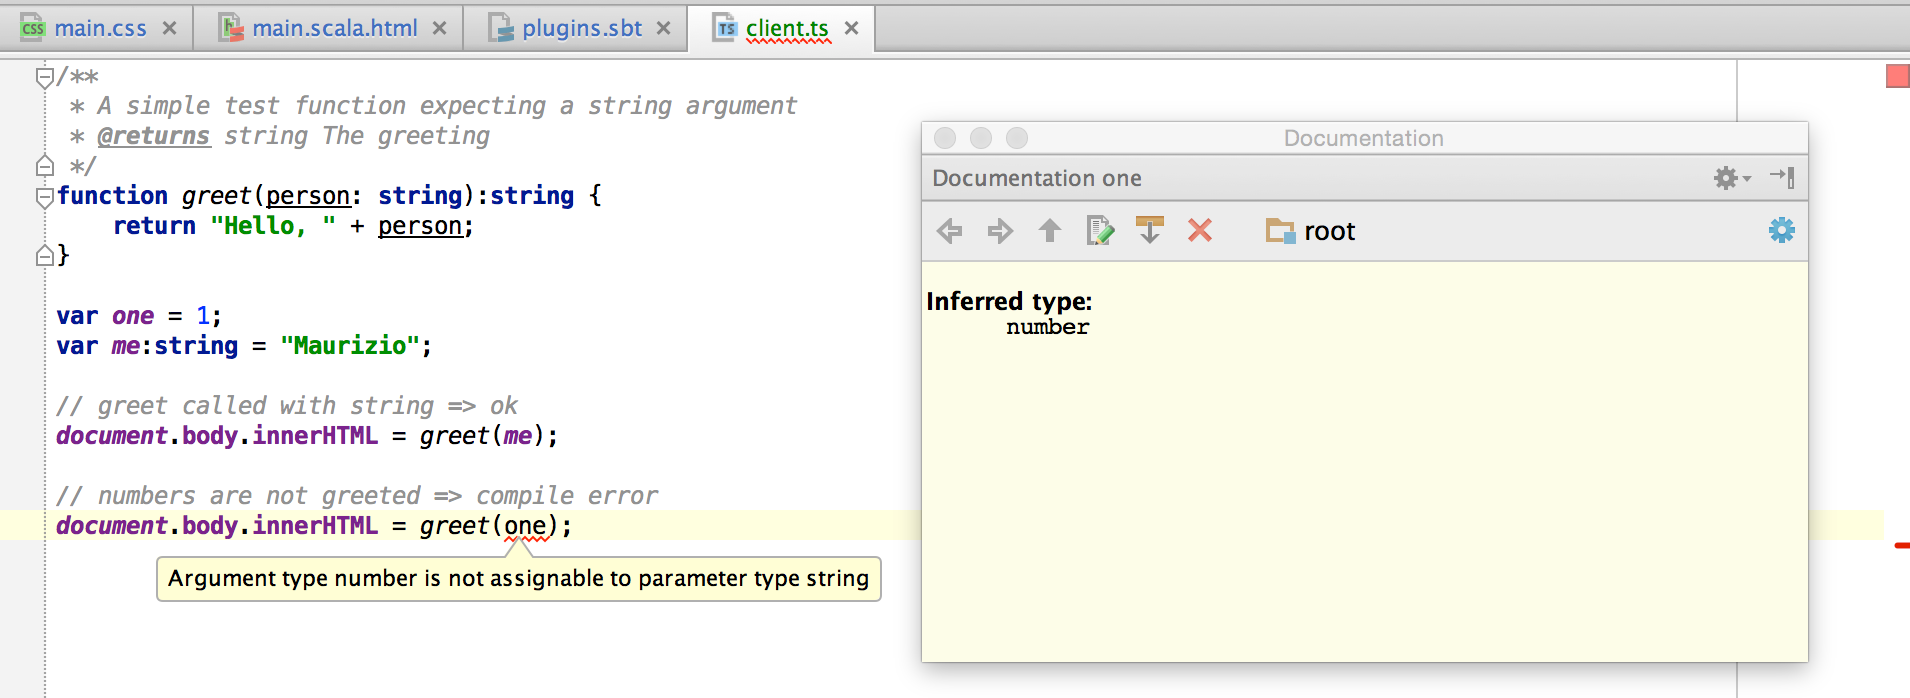
\includegraphics[width=0.9\textwidth]{typescript-idea.png}
\caption{TypeScript in IntelliJ IDEA}
\end{figure}

While these solutions, and especially TypeScript, smooth out the main flaws of JavaScript and are being adopted by a rising number of developers, they do not solve the need to create redundancy in client/server web applications. So for this work, I continued to search for a solution to both problems.

\subsubsection{Unified Programming Language for Server and Client Code}

There are several attempts to bring JavaScript on the server, and the most popular is Node.js, which was released in 2009. While there surely are some scenarios for server-side JavaScript like screen-capturing of rendered websites, in my opinion this is the wrong way of language unification. It brings the problems connected to JavaScript to the server side, where much better designed languages exist, like Scala. 

The other way around would be the perfect solution: Using a rich and well engineered language to write server and client code. So after some research I found the Scala.js project \cite{scalajs}. It was started on February 2013 by Sébastien Doeraene, a member of the Scala team at LAMP (Programming Methods Laboratory at EPFL), after Martin Odersky suggested him to work on a JavaScript compiler \cite{scalajs-interview}.

Scala.js ports most parts of Scala and it's standard library to the browser, compiling Scala to JavaScript or more precisely to ECMAScript 5.1. So, among others, it is possible to use Scala collections, classes and traits, types, pattern matching and even Futures for concurrent processing. 

%TODO2 scala lib results in 32 mb ECMAScript, google compiler removing dead code <200kb, benchmarks

Beside avoiding to use ECMAScript directly, the big advantage of using Scala.js is beeing able to cross-compile parts of the same Scala code for both the server-side JVM and the browser-side ECMAScript engine. This helps reducing redundancy and is especially helpful for data transfer objects (DTO) representing entities of the respective domain, in the case of the CA Guide sites, areas and beacons, as we will see later.

On 5th February 2015, at the time of this writing and exactly two years after this project was started, the release v0.6.0 was announced on the official Scala website and the experimental flag was removed, defining Scala.js "production-ready" \cite{scalajs06}.

So I decided to try this very promising compiler for the CA Guide back end.

\section{Setting up the Development Platform}

\subsection{Project Structure, Scala and Play}

Typesafe's Play web framework %TODO see section bla
 is used as basis for developing the CA Guide back end. It is installed using the Activator tool, which acts as build tool and dependency manager.
 
The project is configured according to the "Play! application with Scala.js" skeleton \cite{playscalajs} referenced on the Scala.js homepage, splitting it up into three subprojects:

\begin{description}[leftmargin=!,labelwidth=\widthof{\bfseries editor-server}]
\item[$\bullet$ editor-server] The Play project including server side Scala code and the typical Play application structure consisting of an app folder%TODO
\item[$\bullet$ editor-client] Client only source code, the Scala.js project
\item[$\bullet$ editor-shared] Shared Scala sources, accessible from both the client and server source code
\end{description} 
 
The project was imported in IntelliJ IDEA 14 as sbt project, which worked very well without major problems. 

Using the activator command in a shell, %TODO run - start webserver and rebuild on page refreh, test command executes the tests

\subsection{Adding Reactive Couchbase as Scala Database Driver}

ReactiveCouchbase is an open-source database driver for connecting a Couchbase database to a Scala program \cite{reactivecouchbase}. Queries are performed using the elegant Scala Future paradigm, that will be discussed later in detail. For the integration with a Play application, a dedicated plugin is available.

Plugins can be added to Play by defining the name, version and if needed the repository url to the build.sbt file. This dependency has only to be added to the server project's dependencies.

\begin{lstlisting}[caption={Adding ReactiveCouchbase to Play via build.sbt},basicstyle=\tiny\ttfamily,language=c,aboveskip=15pt]
libraryDependencies += "org.reactivecouchbase" %% "reactivecouchbase-play" % "0.3"
resolvers += "ReactiveCouchbase" at "https://raw.github.com/ReactiveCouchbase/repository/master/releases"
\end{lstlisting}

To activate the plugin, a line has to be added to conf/play.plugins, where the first element defines the activation order and the second denotes the plugin.

\begin{lstlisting}[caption={Activating the plugins via play.plugins},basicstyle=\tiny\ttfamily,language=c,aboveskip=15pt]
\small\ttfamily{400:org.reactivecouchbase.play.plugins.CouchbasePlugin}
\end{lstlisting}

Now the connection to a previously installed Couchbase Server has to be configured. A Couchbase bucket named "guide-editor" was created using the database's admin console.

\begin{lstlisting}[caption={Attaching the driver to the local Couchbase Server},basicstyle=\tiny\ttfamily,language=c,aboveskip=15pt]
couchbase {
  buckets = [{
    host="127.0.0.1"
    port="8091"
    base="pools"
    bucket="guide-editor"
    user="<user>"
    pass="<pass>"
    timeout="0"
  }]
}
\end{lstlisting}

\subsection{Adding µPickle as Lightweight Serialization Framework}

µPickle (pronounced micro-Pickle) is a lightweight open source serialization/deserialization\footnote{serialization/deserialization is also called pickling/unpickling, explaining the framework's name} framework developed by Li Haoyi \cite{upickle}.
It works on the server side JVM as well as in the Scala.js browser part, making it's a good fit for transferring objects between the client and the server in this project. This is achieved by avoiding reflection in favor of performance, depending on nothing but the standard library on the Scala.js part.

For enabling it, a dependency has to be added to both the client and the server projects in the build.sbt file.

\begin{lstlisting}[caption={Adding a dependency to the client and server project},basicstyle=\tiny\ttfamily,language=c,aboveskip=15pt]
resolvers += "bintray/non" at "http://dl.bintray.com/non/maven"
# client
libraryDependencies += "com.lihaoyi" %%% "upickle" % "0.2.8"
# server
libraryDependencies += "com.lihaoyi" %% "upickle" % "0.2.8"
\end{lstlisting}

Note the new "\%\%\%" operator, which adds the Scala.js version to the artifact name to be retrieved, extending the regular sbt "\%\%" operator that adds the Scala version.

\subsection{Adding Bootstrap as UI Framework}

Bootstrap is a popular open source web UI library, started by two Twitter engineers in 2011 \cite{bootstrap}, providing a rich set of UI components like buttons, dropdowns, glyphs and modal dialogs in the browser. It consists primarily of cascading style-sheets (css), a font containing the glyphs for common actions and optional JavaScript extensions for programmed behavior.

After adding the bootstrap.css to Play's folder "public/css" and the glyph fonts to the "public/fonts" folder of the Play application, the components can be used by creating HTML elements assigned to the desired css classes and matching the needed structure of the respective UI component.

\subsection{Activating the Less Compiler}

Cascading style sheets are the common way to separate design and data of web sites and applications. Less is a meta language on top of css, Link
evolution step of standard css files, adding missing concepts to write more concise and better readable css-code. It was started in 2009 as open-source project by Alexis Sellier \cite{less}.

After enabling less, assets can be placed under assets/less and are automatically compiled to regular css files with the regular 'compile' command or when an automatic rebuild is triggered by a browser page refresh after changing a file.
%less as css


\section{Architecture and Design}

\subsection{Overview}

%Single page,  

\subsection{The Controller}

\subsubsection{Designing the REST HTTP Interface}

%HTTP methods
%Excerp routing file, reverse routing, single place of definition

\subsubsection{Controller Actions}


\subsection{The Model}

\subsubsection{Designing Classes to Cross-Compile}

%ClassDTO + Class, implicit conversion to Class: val site:Site = siteDTO, site.save() 

\subsubsection{Creating NoSQL Design Documents}

\subsubsection{Accessing the Database using Scala Futures}

The interface of the Reactive Couchbase Driver makes extensive use of Futures, a language feature introduced in Scala 2.10\footnote{The most recent Edition of \cite{scala-book} at the time of writing doesn't cover Scala 2.10. A more detailed description of Futures can be found in the Scala Online Documentation \cite{scala-futures}.}.

In this section the Future concept is explained using a simple query which retrieves a list of all sites stored in the guide-editor Couchbase bucket.


\subsection{The View}

\subsubsection{Play HTML Templates}

\subsubsection{Mockups}

\subsubsection{The Client code in Scala.js}

%Own MVC, the Model acts as a kind of local cache. Resorting, filtering
%Controller generates call to the REST Interface


 
% Chapter 6

\chapter{Example Site Model} % Main chapter title

\label{systemrev} % For referencing the chapter elsewhere, use \ref{Chapter1} 

\lhead{Chapter 6. \emph{System Review}} % This is for the header on each page - perhaps a shortened title

%----------------------------------------------------------------------------------------

\section{Introduction}

%Serves as Evaluation and Example

\section{Modelling the Tech Center}

\subsection{Indoor Modelling}

\subsection{Outdoor Modelling}


\section{Testing the CA Guide Front End}


\section{Analytics with the CA Guide Back End} 
% Chapter 7

\chapter{Conclusion} % Main chapter title

\label{conclusion} % For referencing the chapter elsewhere, use \ref{Chapter1} 

\lhead{Chapter 7. \emph{Conclusion}} % This is for the header on each page - perhaps a shortened title

%----------------------------------------------------------------------------------------

\section{Contribution}

\section{Future Work} 

%----------------------------------------------------------------------------------------
%	THESIS CONTENT - APPENDICES
%----------------------------------------------------------------------------------------

\addtocontents{toc}{\vspace{2em}} % Add a gap in the Contents, for aesthetics

\appendix % Cue to tell LaTeX that the following 'chapters' are Appendices

% Include the appendices of the thesis as separate files from the Appendices folder
% Uncomment the lines as you write the Appendices

% Appendix A

\chapter{A Tiny DSL in Scala} % Main appendix title

\label{AppendixA} % For referencing this appendix elsewhere, use \ref{AppendixA}

\lhead{Appendix A. \emph{A Tiny DSL in Scala}} % This is for the header on each page - perhaps a shortened title

\begin{lstlisting}[caption={Building.scala},basicstyle=\small\ttfamily,language=c,aboveskip=15pt]

import shared.model.Coordinates

/**
 * Tiny Internal DSL for defining buildings
 * Maurizio Tidei, 2015.
 */
class Building {

  // The south-west corner
  var sw: Option[Coordinates] = None

  // The north-east corner
  var ne: Option[Coordinates] = None

  // A map floor number -> floorplan image name
  var floors = Map[Int,String]()

  /**
   * Defines the south-west corner
   * @param coord The south-west Coordindates
   */
  def placedAtSouthWest(coord: Coordinates) = {

    sw = Some(coord)
    this
  }

  /**
   * Defines the north-east corner
   * @param coord The north-east Coordinates
   * @return
   */
  def andNorthEast(coord: Coordinates) = {

    ne = Some(coord)
    this
  }

  /**
   * Adds a floor
   * @param floor a tuple combining the floor number to a floorplan image name
   */
  def using(floor: (Int, String)) = {

    floors += (floor._1 -> floor._2)
    this
  }
}

/**
 * Helper class for implicit conversion of Strings
 * @param floorImageName
 */
class FloorImage(floorImageName: String) {

  /**
   * Creates a tuple combining the floorImageName with the floor number
   * @param number The floor number
   * @return tuple for Building's using method
   */
  def asFloor(number: Int) = {

    (number, floorImageName)
  }
}

/**
 * Companion object
 */
object Building {

  // Defines the implicit conversion from String to FloorImage
  implicit def stringToFloorImage(floorImageName: String) = new FloorImage(floorImageName)

  // A list of buildings
  val list = List(

  // Techcenter Park 31
  new Building  placedAtSouthWest Coordinates(47.652374, 9.167594)
                andNorthEast      Coordinates(47.652580, 9.168151)
                using ("park31-attic-floor"   asFloor 3)
                using ("park31-1st-floor"     asFloor 2)
                using ("park31-1st-floor"     asFloor 1)
                using ("park31-ground-floor"  asFloor 0)

  )
}
\end{lstlisting}

\begin{lstlisting}[caption={Coordinates.scala},basicstyle=\small\ttfamily,language=c,aboveskip=15pt]

/**
 * A geographic coordinate pair
 *
 * @param lat The latitude
 * @param lon The longitude
 * Maurizio Tidei, 2015.
 */
case class Coordinates(var lat: Double, var lon: Double) {


  /**
   * Add two coordinates
   * @return the resulting Coordinate
   */
  def +(that: Coordinates): Coordinates = {

    return Coordinates(this.lat + that.lat, this.lon + that.lon)
  }


  /**
   * Multiply a coordinate with a tuple of two doubles
   * @return the resulting Coordinate
   */
  def *(tuple: Tuple2[Double, Double]): Coordinates = {

    return Coordinates(this.lat * tuple._1, this.lon * tuple._2)
  }

}
\end{lstlisting}


%\input{Appendices/AppendixB}
%\input{Appendices/AppendixC}

\addtocontents{toc}{\vspace{2em}} % Add a gap in the Contents, for aesthetics

\backmatter

%----------------------------------------------------------------------------------------
%	BIBLIOGRAPHY
%----------------------------------------------------------------------------------------

\label{Bibliography}

\lhead{\emph{Bibliography}} % Change the page header to say "Bibliography"

% natbib
%\bibliographystyle{unsrtnat} % Use the "unsrtnat" BibTeX style for formatting the Bibliography
%\bibliography{Bibliography} % The references (bibliography) information are stored in the file named "Bibliography.bib"

% biblatex
\printbibheading
\printbibliography[nottype=url,heading=subbibliography,title={Books and Papers}]
\printbibliography[type=url,heading=subbibliography,title={Web Sources}]

\end{document}
  